\chapter{Desenvolvimento}\label{chp:desenvolvimento}

Para realização da solução proposta nesse trabalho, é necessário o desenvolvimento de um aplicativo móvel para que o rastreamento de doenças infecciosas ocorra de forma automática. Assim, na Seção \ref{sec:requisitos} são apresentados os requisitos funcionais e não funcionais do sistema, junto com a análise de cada um deles. A Seção \ref{sec:modelagem} tem o propósito de apresentar todo o processo de modelagem do sistema, discutindo sobre o racional por trás de cada modelagem e apresentando os diagramas construídos. Na Seção \ref{sec:uiux} são apresentadas as interfaces construídas para o aplicativo. A Seção \ref{sec:implementacao} contém a implementação das interfaces do usuário, modelagens e infraestrutura do sistema, utilizando o fluxo de trabalho \textit{GitFlow}.

\section{Levantamento e Análise de Requisitos}\label{sec:requisitos}
O aplicativo deve automatizar todo o ciclo do rastreamento, desde a captura da exposição à uma doença, até a notificação feita à pessoa possivelmente exposta. Com isso, a partir do problema de rastreamento de contatos apresentado no Capítulo \ref{chp:Introducao}, o processo de análise de requisitos foi feito pensando nos possíveis casos de uso do usuário.

Começando pelos requisitos não funcionais, a eficácia da solução depende diretamente do número de usuários que utilizarem o aplicativo. Isso significa que quanto mais tipos de dispotivos móveis forem suportados, mais potenciais usuários o aplicativo pode alcançar. Por conta disso, o aplicativo pode ser desenvolvido especialmente para cada tipo de \Sigla{Sistema Operacional}{SO} ou utilizando um \textit{framework} híbrido, em que a partir da mesma base de código é possível construir os arquivos para cada SO.

Levando em consideração o tempo de desenvolvimento do aplicativo e o número de pessoas envolvidas, a utilização de um \textit{framework} híbrido é a melhor forma para atingir o maior número de usuários.

Além disso, como o aplicativo armazena os dados de localizações dos usuários, ele deve se preocupar em garantir a segurança dos mesmos. Essa segurança será garantida a partir da utilização de criptografia. Ela será aplicada aos dados em trânsito, ou seja, durante a comunicação entre cliente e servidor.

Ainda relacionado à segurança, a fim de preservar a privacidade das pessoas que utilizarem o aplicativo, a aplicação ou os usuários não devem ser capazes de descobrir quem possivelmente expôs outras pessoas à alguma doença. Isso significa que quando um usuário receber uma notificação de exposição, ele não será capaz de identificar quem foi, nem o local que isso ocorreu. Para isso, o aplicativo não terá a inserção de nenhum dado pessoal, ou seja, a autenticação será feita de forma anônima, onde cada usuário será representado por uma cadeia de caracteres aleatórios.

Por último, toda localização terá prazo de validade de 14 dias. Isso significa que todo local visitado pelo usuário será armazenado apenas durante esse prazo. Como a solução do problema é a automação do rastreamento de contatos, localizações mais antigas do que esses dias não são necessárias, já que o período de contágio e transmissão do vírus haveria terminado.

A partir do que foi explicado nos parágrafos anteriores, a Tabela \ref{tab:tabelanf} elenca os três requisitos não funcionais e suas respectivas prioridades, que podem ser obrigatórias, importantes ou opcionais.

\begin{table}[!htb]
\caption[Tabela de requisitos não funcionais]{Requisitos não funcionais}
\label{tab:tabelanf}
\begin{center}
\begin{tabular}{|l|l|l|}
\hline
\multicolumn{1}{|c|}{\textbf{Código}} & \multicolumn{1}{c|}{\textbf{Nome}}            & \multicolumn{1}{c|}{\textbf{Prioridade}} \\ \hline
RNF01                                 & Compatibilidade multiplataforma               & Opcional                                 \\ \hline
RNF02                                 & Garantia de privacidade e segurança dos dados & Obrigatório                              \\ \hline
RNF03                                 & Exclusão de localizações antigas              & Importante                               \\ \hline
\end{tabular}
\end{center}
\end{table}

Como o aplicativo usará um \textit{framework} multiplataforma para atender os requisitos não funcionais citados anteriormente, essa escolha trás um malefício: recursos nativos de cada dispositivo, como por exemplo o \textit{Bluetooth}, não possuem o mesmo suporte caso fosse uma codificação utilizando uma linguagem nativa.

Levando isso em consideração, os contatos que eventualmente ocorrerem entre diferentes usuários do aplicativo podem ser rastreados a partir de duas principais formas: 

\begin{itemize}
  \item Armazenamento dos locais visitados pelos usuários utilizando um sistema de \textit{check-in}, onde o usuário fará a inserção do local visitado utilizando um sistema de busca;
  \item Armazenamento dos contatos que foram efetuados utilizando o \textit{Bluetooth}. O dispositivo detectará os sinais transmitidos ao seu redor, e fará a persistência desses contatos;
\end{itemize}

Ambas soluções solucionam o problema de formas distintas, porém, levando em consideração o requisito de compatibilidade multiplataforma e do baixo acesso à recursos nativos pelos \textit{frameworks}, a solução utilizada neste trabalho será a partir do sistema de \textit{check-in}.

Com isso, os usuários necessitam de um buscador para encontrar os locais que foram visitados. Esse buscador deve estar relacionado a um extenso BD para que a maioria dos locais inseridos pelos usuários sejam encontrados. Por conta disso, um BD externo deve ser utilizado, já que a criação de um novo não traria a experiência esperada para o usuário.

Depois que a busca foi feita, o usuário deve ser capaz de salvar o local encontrado. O salvamento deve ser feito em um BD remoto, para que a rotina de checagem do rastreamento de contatos seja feita no servidor. Com isso, o dispositivo móvel do usuário não precisará de conectividade com a \textit{Internet}, nem que o aplicativo rode em segundo plano durante a execução da rotina, evitando o consumo desnecessário de dados e de bateria do dispositivo.

Se um usuário for infectado por uma doença, ele deve ser capaz de declarar no aplicativo que está infectado. A partir disso, a rotina de rastreamento de contatos deve ser capaz de relacionar os locais do usuário infectado com os usuários comuns, procurando por algum possível contato que possa ter ocorrido.

O usuário deve receber notificações caso o mesmo tenha tido algum possível contato com outras pessoas que utilizam o aplicativo e estavam infectadas. Essa notificação deve ser enviada de forma automática e sem a necessidade de intervenção humana, para que o problema seja resolvido de forma automática de ponta a ponta.

Para melhor usabilidade, é importante que o usuário consiga visualizar o local que está sendo buscado para confirmar que este é o local desejado para efetuar o \textit{check-in}. Por isso, quando o usuário efetuar a busca de uma localização, a visualização dos detalhes, tais como nome, endereço e fotos, devem estar disponíveis. 

Por último, o usuário deve ser capaz de conseguir visualizar todos os locais e as respectivas datas de visita que foram salvas no aplicativo. Essa funcionalidade não afeta no rastreamento de contatos, mas ajuda na experiência de utilização do aplicativo.

A partir de toda análise acima, foram levantados seis requisitos funcionais que estão representados na Tabela \ref{tab:tabelaf}.

\begin{table}[!htb]
\caption[Tabela de requisitos funcionais]{Requisitos funcionais}
\label{tab:tabelaf}
\begin{center}
\begin{tabular}{|l|l|l|}
\hline
\multicolumn{1}{|c|}{\textbf{Código}} & \multicolumn{1}{c|}{\textbf{Nome}}   & \multicolumn{1}{c|}{\textbf{Prioridade}} \\ \hline
RF01                                  & Buscar localizações                  & Obrigatório                              \\ \hline
RF02                                  & Salvar localizações                  & Obrigatório                              \\ \hline
RF03                                  & Declarar caso de infecção confirmado & Obrigatório                              \\ \hline
RF04                                  & Enviar notificação de exposição      & Obrigatório                              \\ \hline
RF05                                  & Visualizar detalhes da localização   & Importante                               \\ \hline
RF06                                  & Listar locais salvos                 & Opcional                                 \\ \hline
\end{tabular}
\end{center}
\end{table}

\section{Modelagem}\label{sec:modelagem}
O processo de modelagem foi feito desde os aspectos mais abstratos do sistema, utilizando os diagramas de componentes e de pacotes, até os mais específicos, utilizando os diagrama de sequência e de atividades.

Para melhor apresentação e discussão de cada uma das modelagens, elas estão dividas nas subseções abaixo.

\subsection{Modelagem dos componentes do sistema}
A visão geral do sistema desenvolvido é representado pelo diagrama de componentes. Nele são contidos os componentes macros do sistema, como pode ser visto na \Figura{fig:diagramacomponentes}.

\begin{figure}[!htb]
  \centering
  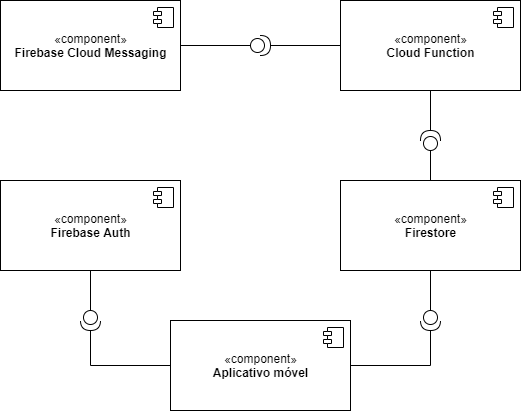
\includegraphics[scale=0.65]{diagrama-de-componentes.png}
  \caption{Diagrama de componentes.}
  \label{fig:diagramacomponentes}
\end{figure}

Cada um dos componentes do diagrama possui uma responsabilidade bem definida. O aplicativo móvel representa a interface do usuário e algumas regras de negócio que foram implementadas nas camadas interiores da \textit{Clean Architecture}.

O \textit{Firebase Auth} é o serviço responsável pela autenticação dos usuários, que nesse caso é utilizada apenas a autenticação anônima, como foi explicado nos capítulos anteriores.

O \textit{Firestore} representa o BD do sistema, que armazenará as localizações visitadas por cada usuário e as que forem classificadas como infectadas.

A \textit{Cloud Function} representa os \textit{scripts} que fazem a análise do rastreamento de contatos e possuem a responsabilidade de ativar o sistema de notificações se algum encontro entre usuários ocorrer.

O \textit{Firebase Cloud Messaging} é o serviço de envio de notificações.

Note que as conexões do diagrama mostram quais são os componentes que acessam as funcionalidades dos outros. Por exemplo, o aplicativo móvel não faz o envio de nenhuma notificação, a responsabilidade dessa tarefa são dos \textit{scripts} das \textit{Cloud Functions}.

\subsection{Modelagem das funcionalidades do sistema}
% Modelagem geral: casos de uso
% Modelagem de cada caso de uso: atividade e sequência
Cada funcionalidade do sistema foi herdada do levantamento de requisitos. Por conta disso, a partir do levantamento da Seção \ref{sec:requisitos}, foi criada a modelagem do diagrama de casos de uso, representado pela \Figura{fig:usecasesdiagram}. É importante ressaltar que este diagrama reflete a listagem de requisitos funcionais da Tabela \ref{tab:tabelaf}.

\begin{figure}[!htb]
  \centering
  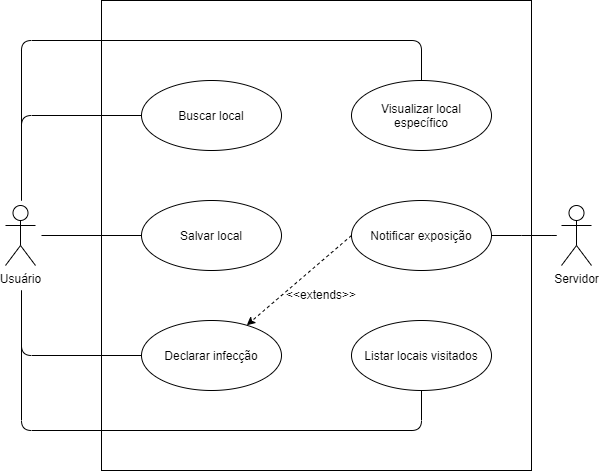
\includegraphics[scale=0.6]{Diagrama de casos de uso.png}
  \caption{Diagrama de casos de uso.}
  \label{fig:usecasesdiagram}
\end{figure}

Como cada caso de uso da \Figura{fig:usecasesdiagram} é uma funcionalidade, os diagramas de atividades e sequência foram modelados para cada um deles. Começando pelo "Buscar local", temos os respectivos diagrama de atividades na \Figura{fig:atividadebuscar} e o de sequência na \Figura{fig:sequenciabuscar}.

\begin{figure}[!htb]
  \centering
  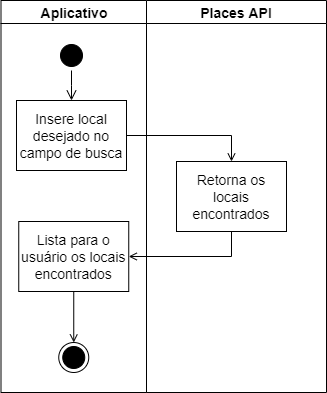
\includegraphics[scale=0.6]{Diagrama de atividades - Buscar.png}
  \caption{Diagrama de atividades da funcionalidade buscar local.}
  \label{fig:atividadebuscar}
\end{figure}

No diagrama de atividades da \Figura{fig:atividadebuscar} o usuário fará consultas em uma das APIs do \textit{Google}, chamada \textit{Places API}. Ela retornará qualquer localização no mundo que corresponda ao texto inserido pelo usuário.

\begin{figure}[!htb]
  \centering
  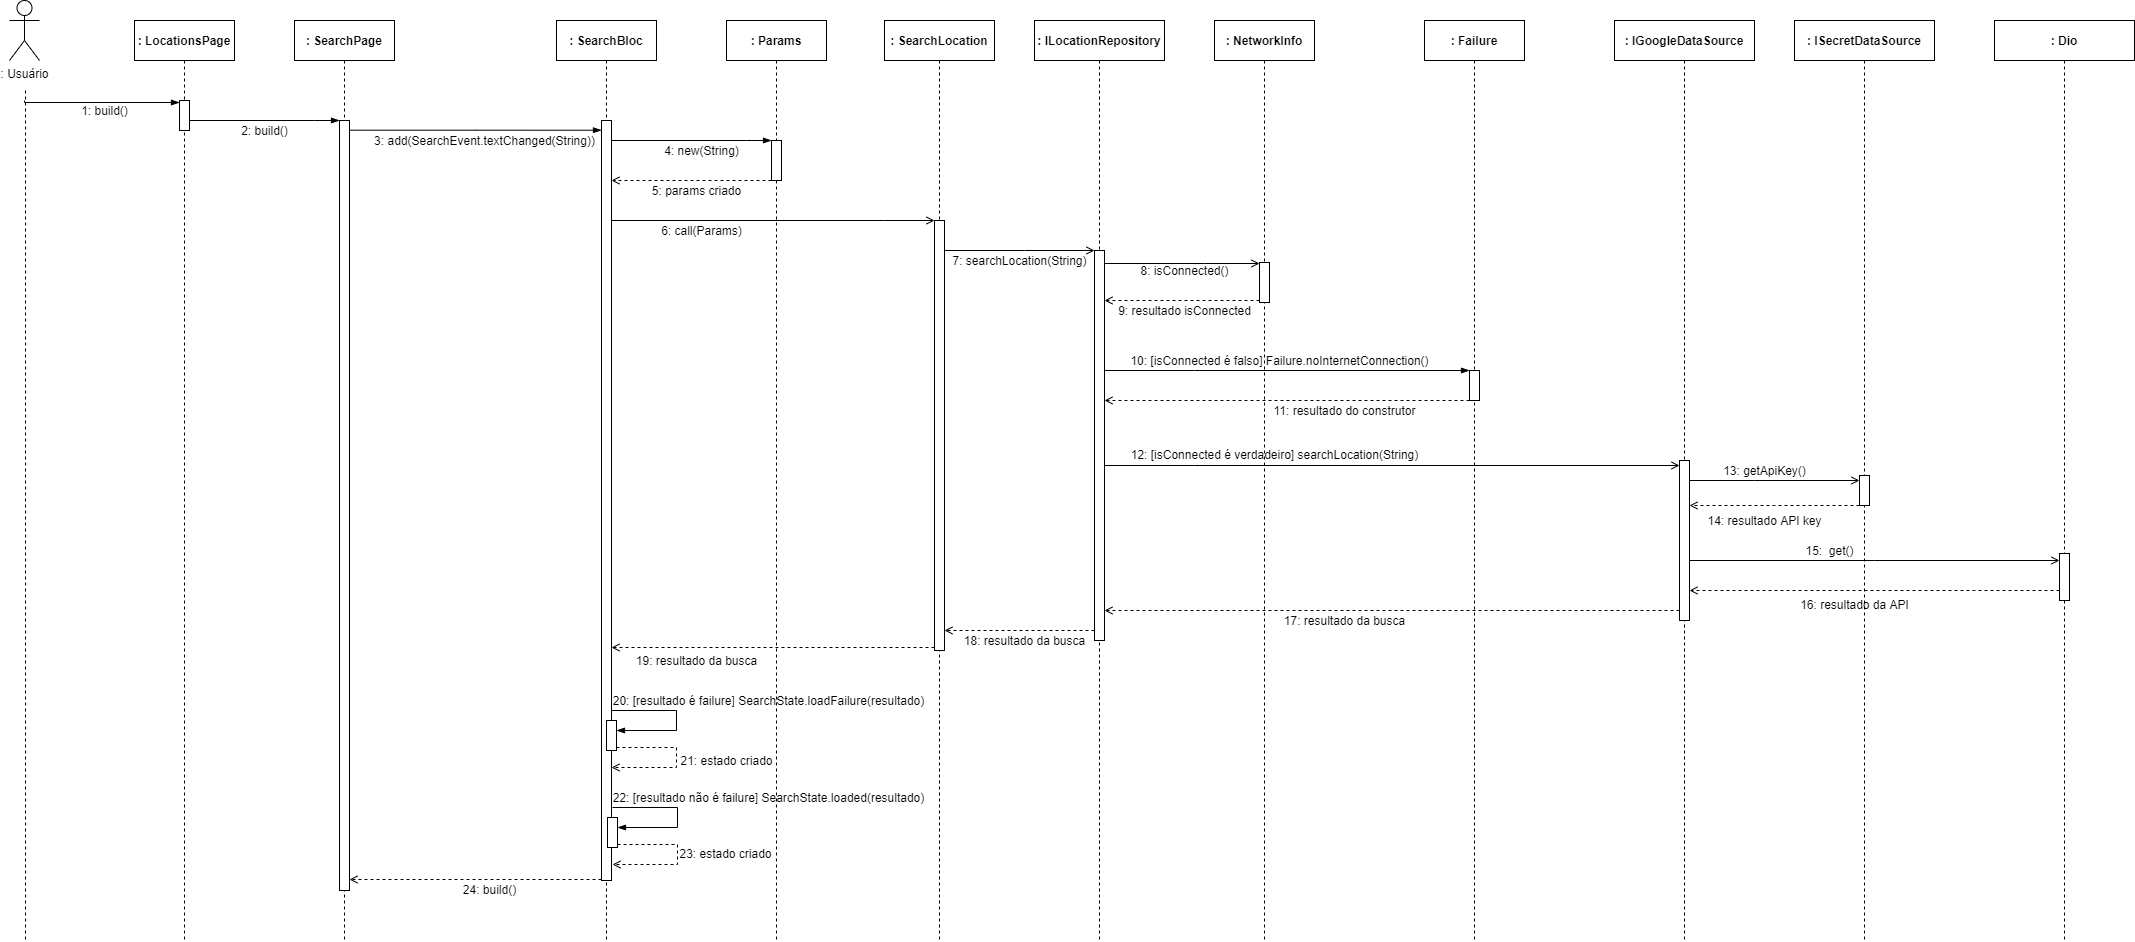
\includegraphics[scale=0.21]{Diagrama de sequencia - Buscar local.png}
  \caption{Diagrama de sequência da funcionalidade buscar local.}
  \label{fig:sequenciabuscar}
\end{figure}

Para a funcionalidade "Salvar local", a \Figura{fig:atividadesalvar} representa o diagrama de atividades, e o de sequência na \Figura{fig:sequenciasalvar}.

\begin{figure}[!htb]
  \centering
  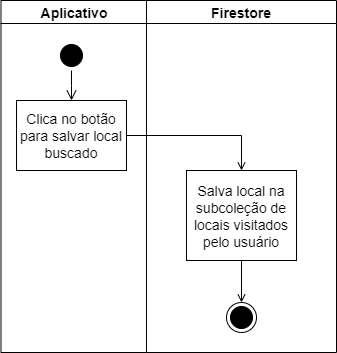
\includegraphics[scale=0.65]{Diagrama de atividades - Salvar.png}
  \caption{Diagrama de atividades da funcionalidade salvar local.}
  \label{fig:atividadesalvar}
\end{figure}

\begin{figure}[!htb]
  \centering
  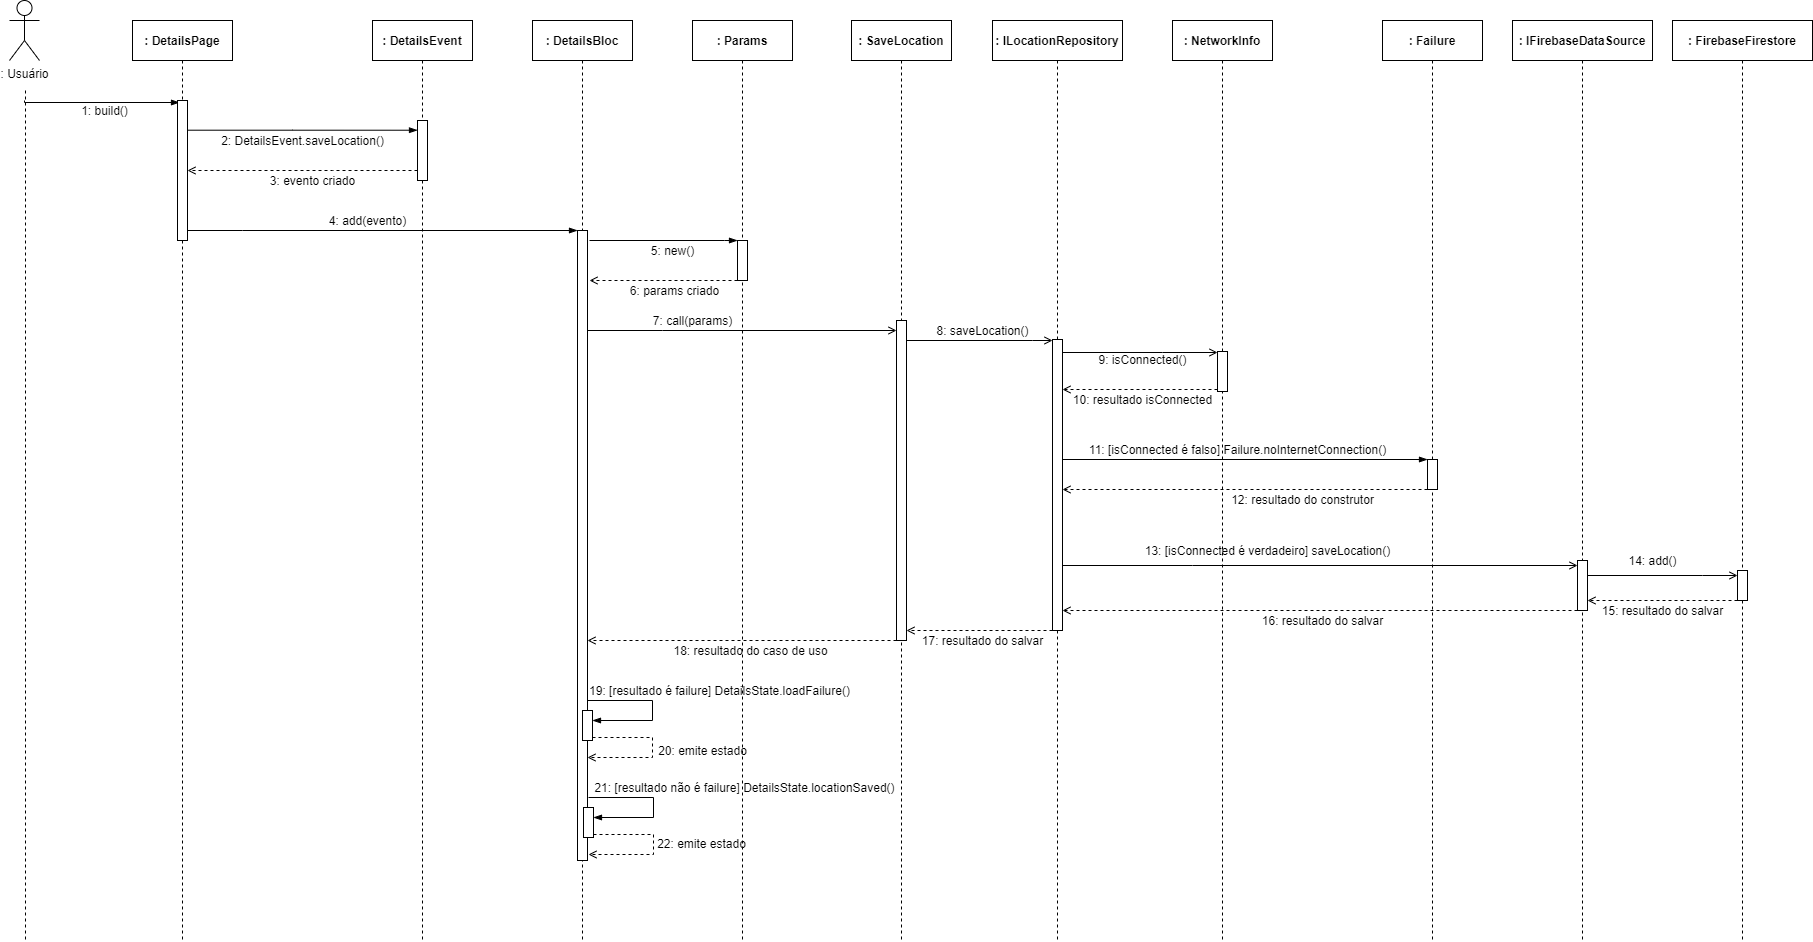
\includegraphics[scale=0.25]{Diagrama de sequencia - Salvar local.png}
  \caption{Diagrama de sequência da funcionalidade salvar local.}
  \label{fig:sequenciasalvar}
\end{figure}



A funcionalidade "Declarar infecção" está representada pelo diagrama de atividades da \Figura{fig:atividadedeclarar} e pelo de sequência da \Figura{fig:sequenciadeclarar}

\begin{figure}[!htb]
  \centering
  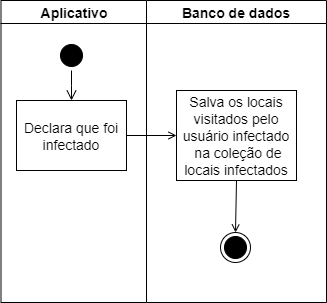
\includegraphics[scale=0.6]{Diagrama de atividades - Declarar.png}
  \caption{Diagrama de atividades da funcionalidade declarar infecção.}
  \label{fig:atividadedeclarar}
\end{figure}

\begin{figure}[!htb]
  \centering
  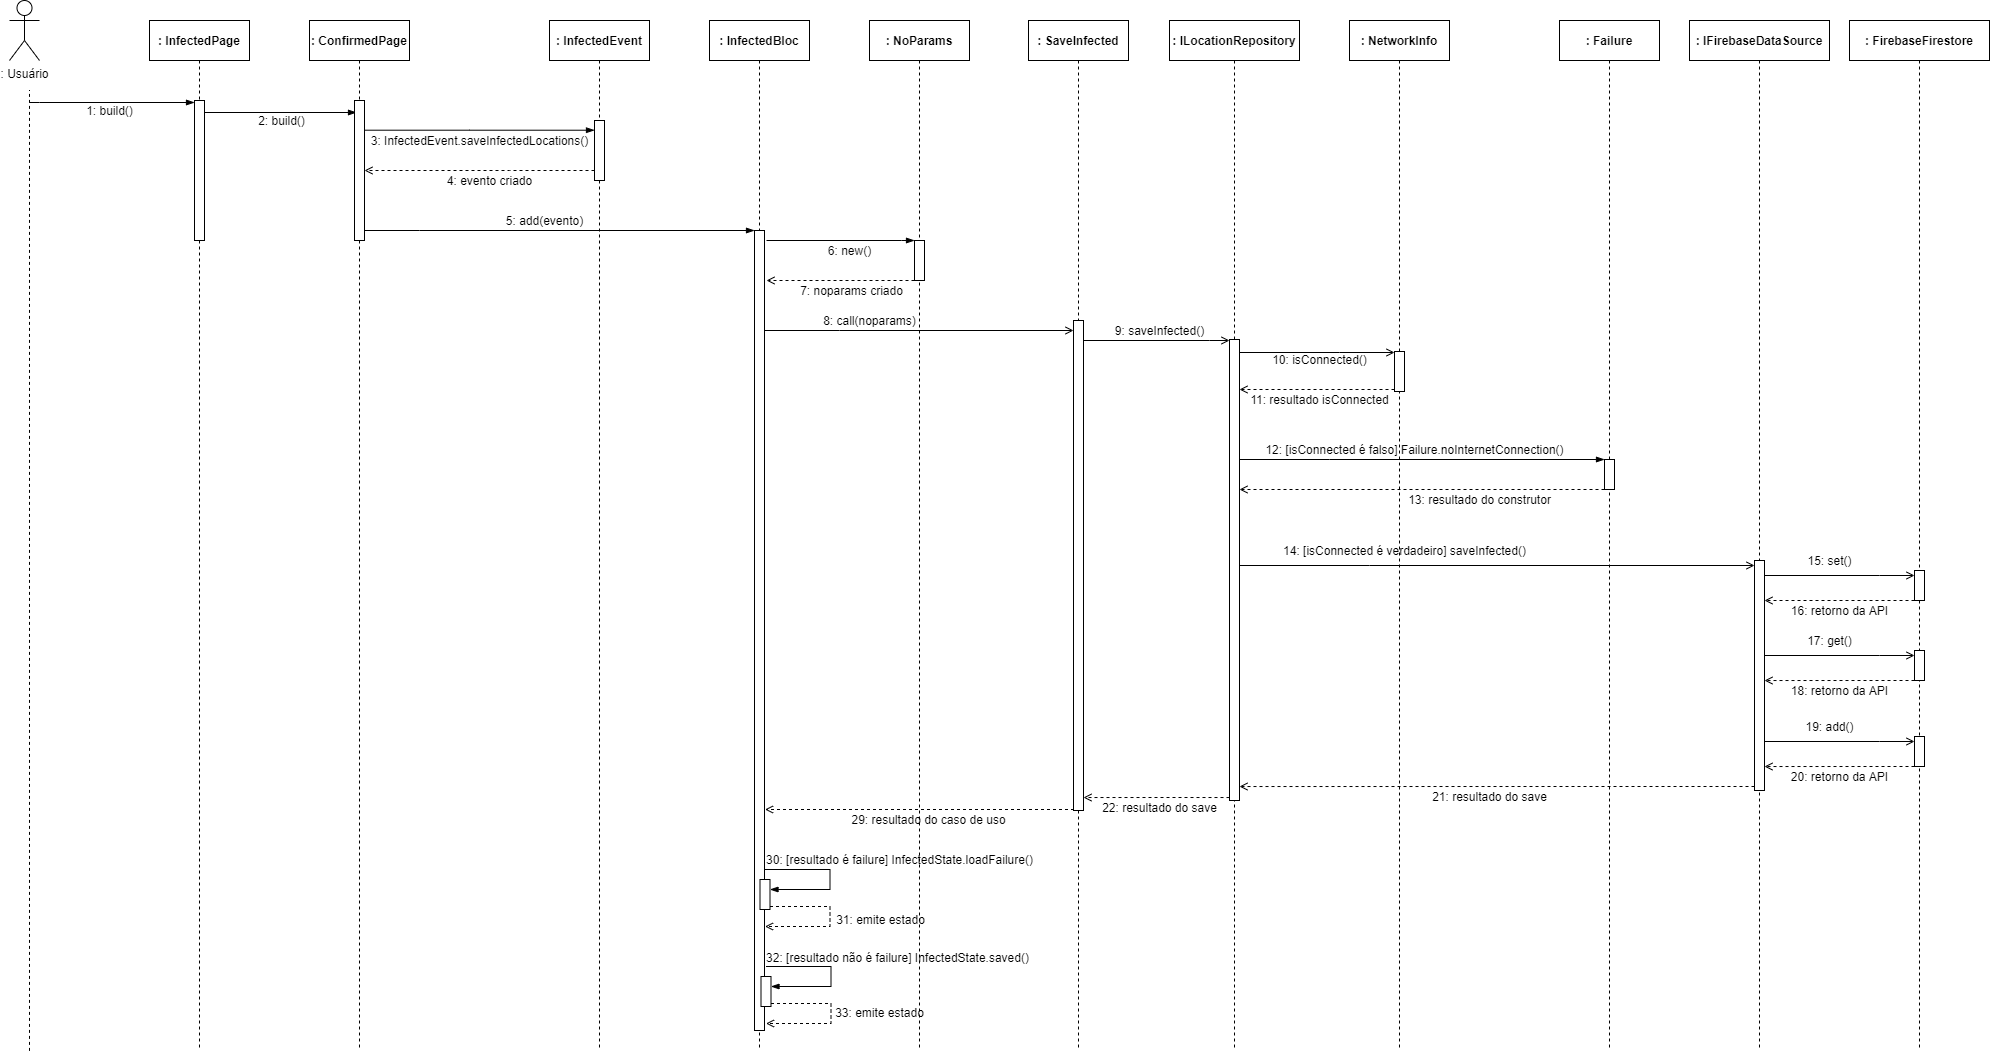
\includegraphics[scale=0.225]{Diagrama de sequencia - Declarar infeccao.png}
  \caption{Diagrama de sequência da funcionalidade declarar infecção.}
  \label{fig:sequenciadeclarar}
\end{figure}

Para a modelagem da funcionalidade "Visualizar local específico" temos a \Figura{fig:atividadevisualizar} para o diagrama de atividades e a \Figura{fig:sequenciavisualizar} para o de sequência.

\begin{figure}[!htb]
  \centering
  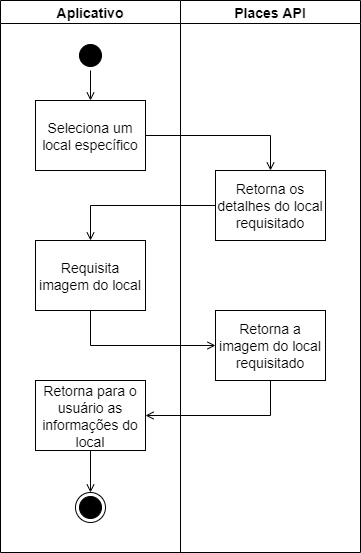
\includegraphics[scale=0.55]{Diagrama de atividades - Visualizar.png}
  \caption{Diagrama de atividades da funcionalidade visualizar local.}
  \label{fig:atividadevisualizar}
\end{figure}

\begin{figure}[!htb]
  \centering
  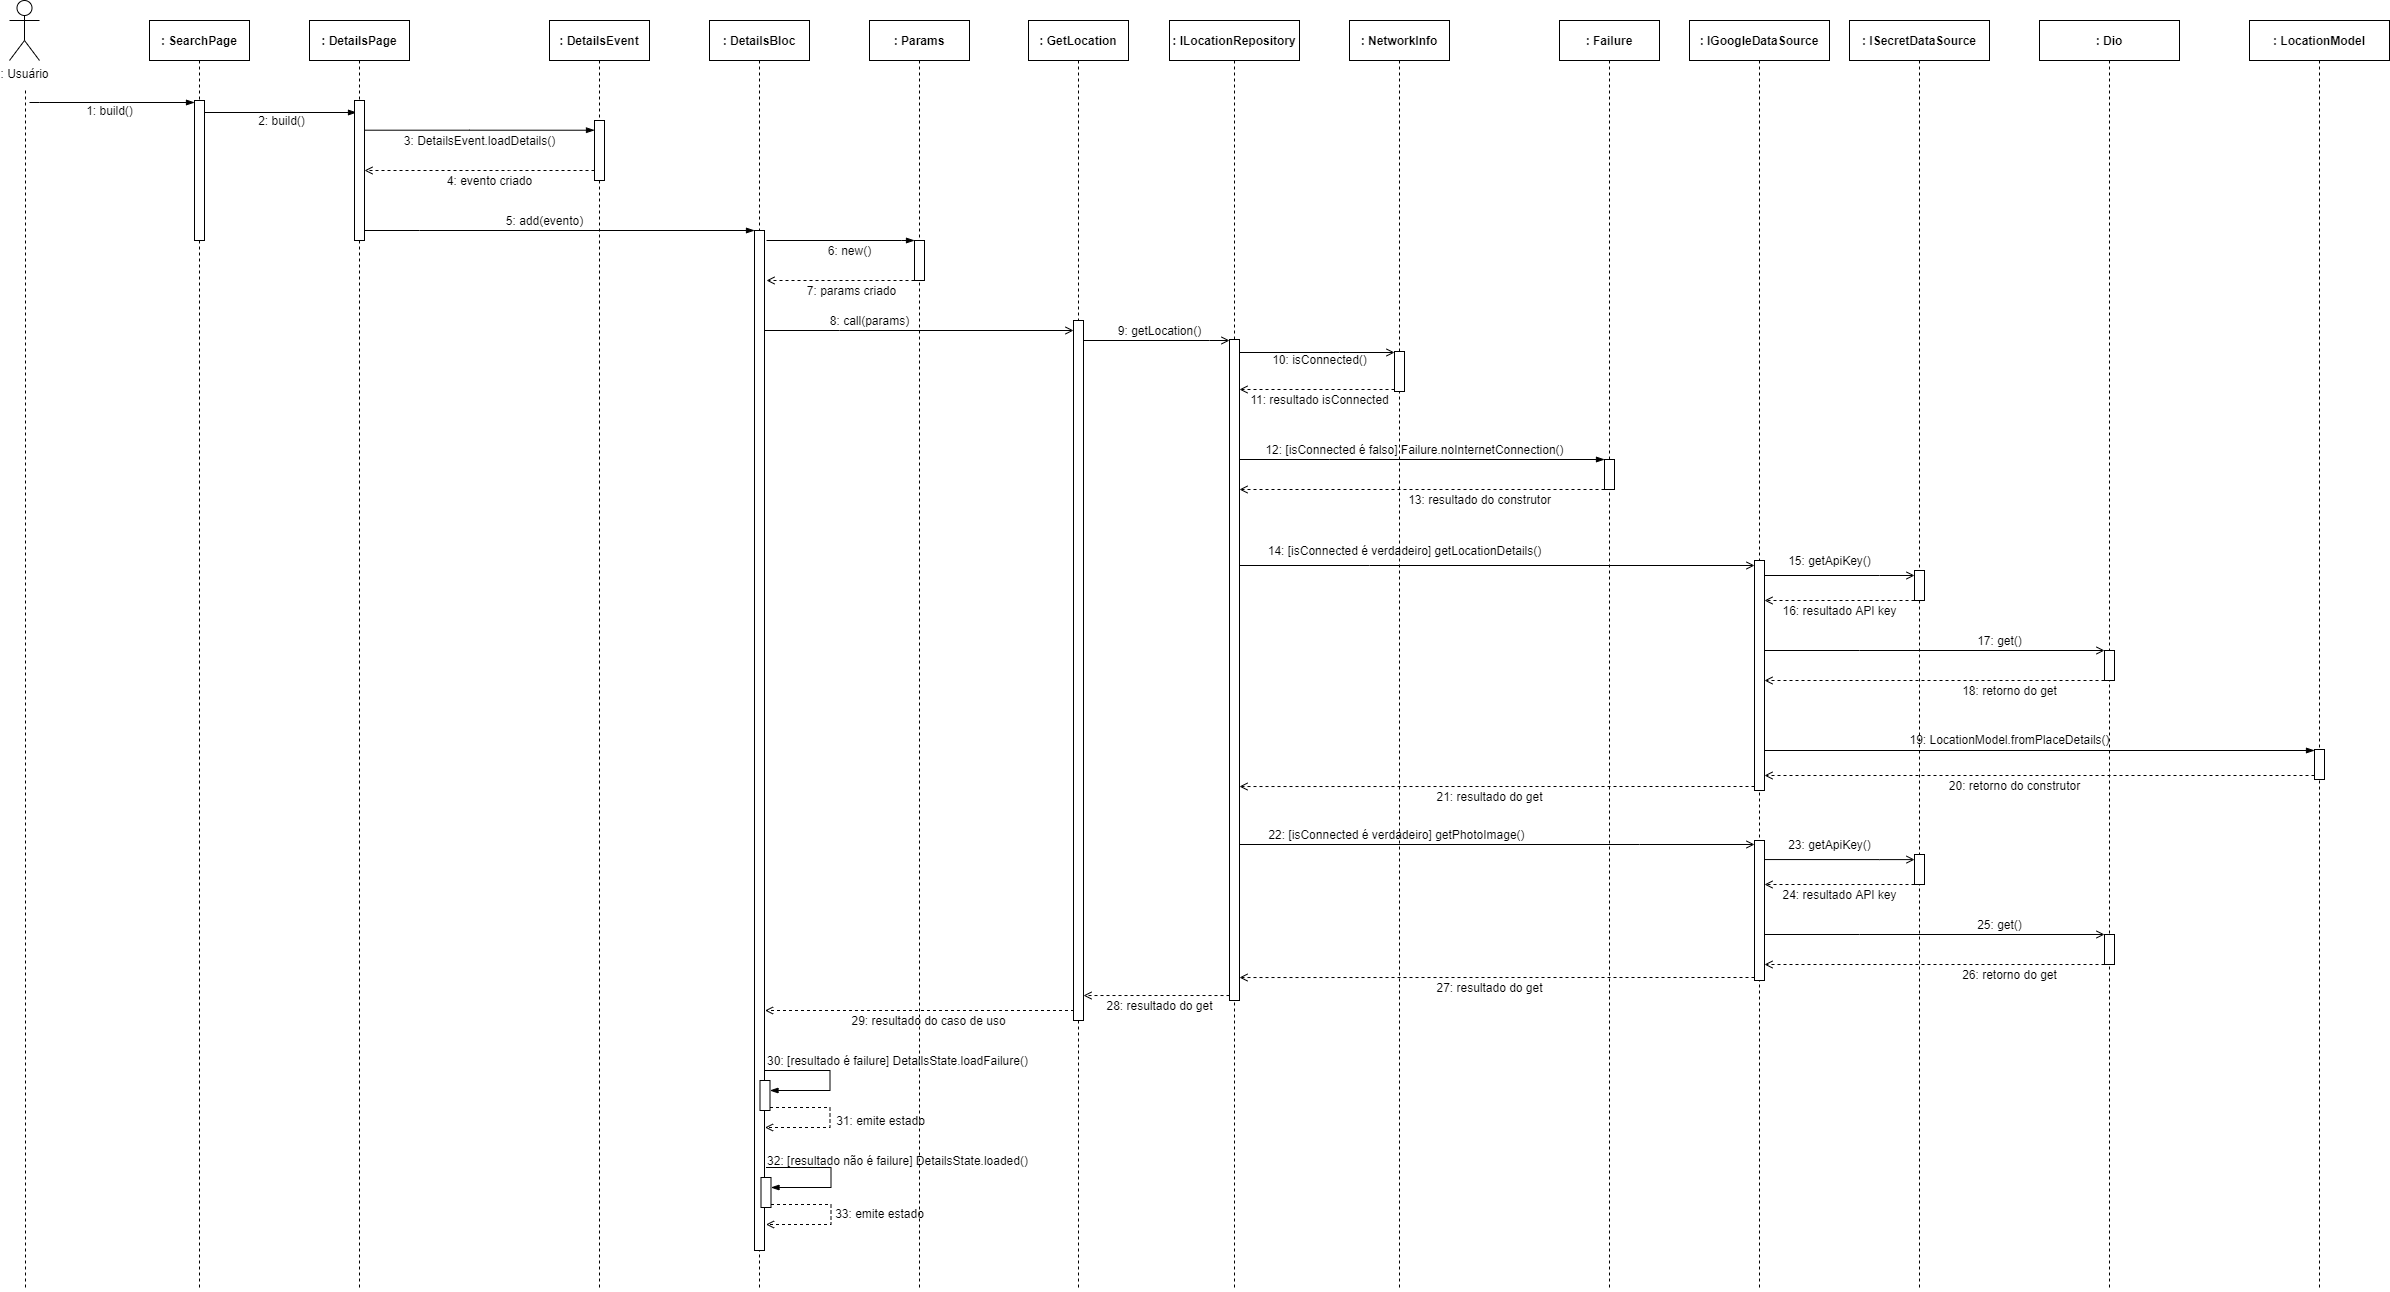
\includegraphics[scale=0.18]{Diagrama de sequencia - Visualizar local.png}
  \caption{Diagrama de sequência da funcionalidade visualizar local.}
  \label{fig:sequenciavisualizar}
\end{figure}

A funcionalidade "Notificar exposição" não possui um diagrama de sequência. Como essa funcionalidade vai ser atendida através do desenvolvimento de \textit{Cloud Functions}, a implementação não utiliza orientação a objetos, será um \textit{script} de análise de encontro entre usuários e não seria bem representado por objetos no diagrama.

Por conta disso, apenas o diagrama de atividades foi modelado e está representado pela \Figura{fig:atividadenotificar}.

\begin{figure}[!htb]
  \centering
  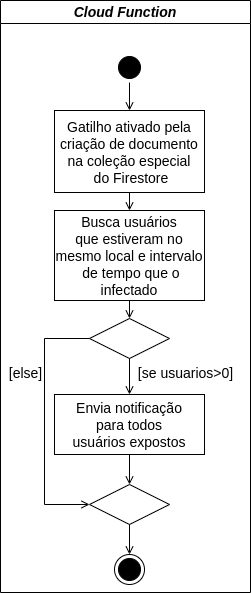
\includegraphics[scale=0.55]{Diagrama de atividades - Notificacao.png}
  \caption{Diagrama de atividades da funcionalidade notificar exposição.}
  \label{fig:atividadenotificar}
\end{figure}

Por último, a funcionalidade "Listar locais visitados" está representada pelo diagrama de atividades e de sequência da \Figura{fig:atividadelistar} e da \Figura{fig:sequencialistar}.

\begin{figure}[!htb]
  \centering
  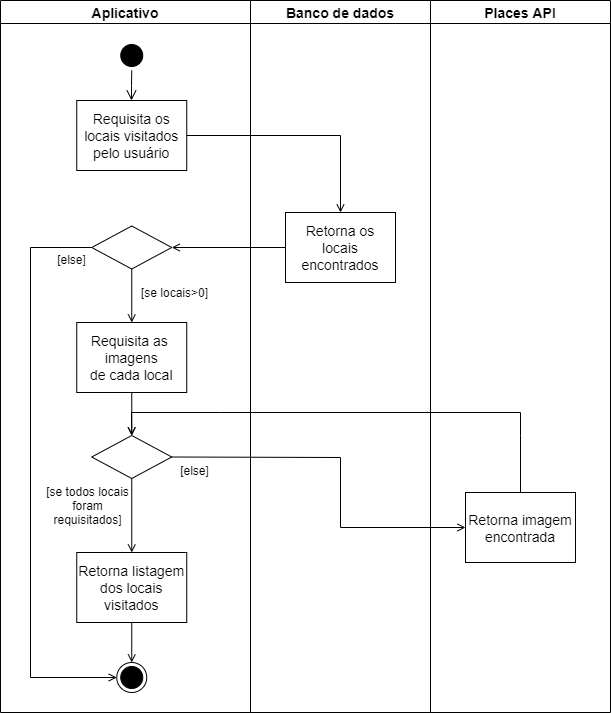
\includegraphics[scale=0.5]{Diagrama de atividades - Listar.png}
  \caption{Diagrama de atividades da funcionalidade listar locais.}
  \label{fig:atividadelistar}
\end{figure}

\begin{figure}[!htb]
  \centering
  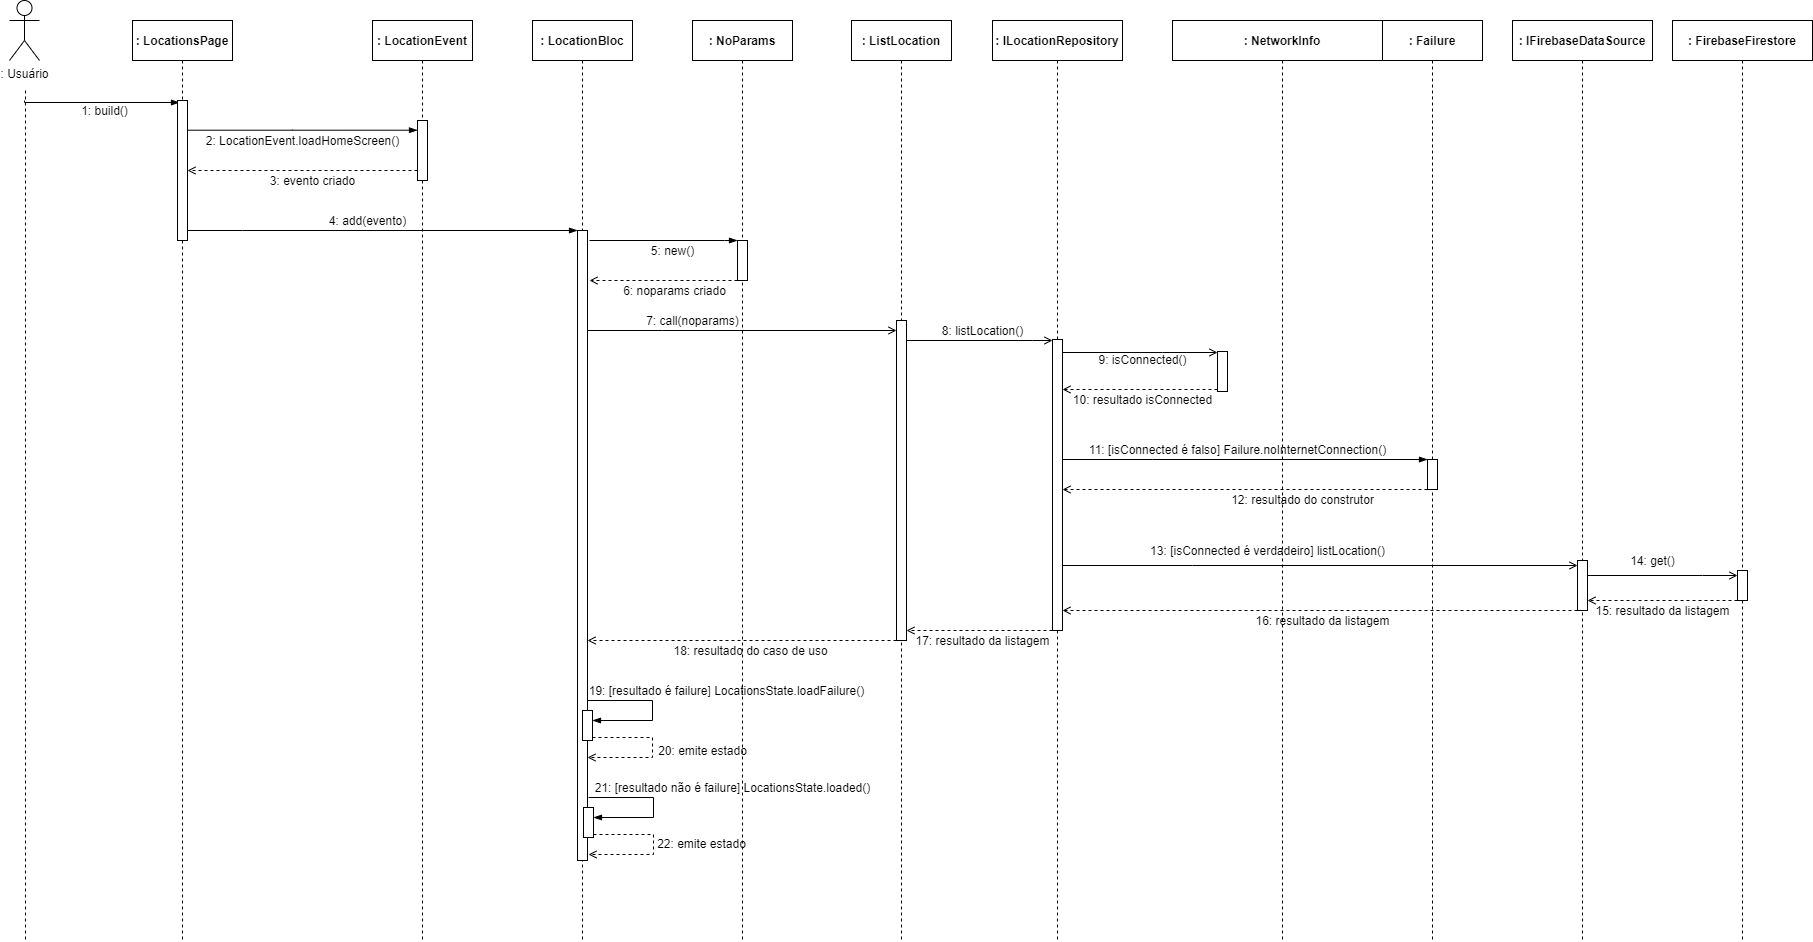
\includegraphics[scale=0.25]{Diagrama de sequencia - Listar locais.png}
  \caption{Diagrama de sequência da funcionalidade listar locais.}
  \label{fig:sequencialistar}
\end{figure}

\subsection{Modelagem da arquitetura do \textit{software}}
Como explicado na Seção \ref{sec:clean}, o aplicativo desenvolvido neste trabalho utiliza os princípios da arquitetura limpa. Por conta disso, a base da arquitetura do \textit{software} é a \Figura{fig:clean1}.

Antes de começar a diagramação, é importante entender a diferença entre dependência e fluxo de dados do aplicativo, porque essa diferença é crucial para que a modelagem não quebre nenhuma das regras da arquitetura limpa.

A dependência do código acontece no tempo de compilação, ou seja, só há dependência entre os componentes se houver uma referência direta para outro componente.

Por exemplo, imagine que em uma das classes da camada \textit{Application Business Rules} do aplicativo possua um caso de uso que em sua implementação exista uma chamada para um método de uma classe presente na camada \textit{Interface Adapters}. Nesse exemplo, o caso de uso possuiria dependência com a camada \textit{Interface Adapters}, e estaria ferindo a regra de dependência, já que essa é uma camada externa em relação à \textit{Application Business Rules}.

Já o fluxo de dados seria equivalente ao fluxo de chamadas dentro do código, que não acontece no tempo de compilação, e sim no de execução. Pode parecer contraditório, mas a dependência nem sempre reflete o fluxo de dados do código.

Utilizando o mesmo exemplo anterior, é possível fazer com que o caso de uso não dependa da camada \textit{Interface Adapters}, mas ainda consiga atingir o mesmo comportamento esperado. Para que isso aconteça, uma interface deve ser criada na camada \textit{Application Business Rules}, e ela conterá as assinaturas dos métodos que o caso de uso necessita. Na camada \textit{Interface Adapters}, uma classe implementará os métodos definidos na interface através do relacionamento de herança.

Dessa maneira, através do \textit{Dependency Inversion Principle}, explicado na subseção \ref{sec:D}, a dependência existirá da camada \textit{Interface Adapters} para a camada \textit{Application Business Rules} por conta da herança, mas no fluxo de chamadas em tempo de execução, será da \textit{Application Business Rules} para a camada \textit{Interface Adapters}.

Com a diferença entre dependência e fluxo de dados compreendida, toda modelagem da arquitetura do sistema deve fazer com que nenhuma camada interna dependa de uma mais externa à ela. Para isso, todas as fronteiras das camadas haverão interfaces para possibilitar a comunicação sem que a regra de dependência seja ferida.

Como o aplicativo fará chamadas para componentes de persistência de dados, utilizando APIs para busca de locais e um BD remoto para o armazenamento, essas chamadas serão realizadas utilizado o padrão de repositório. A partir disso, o fluxo dos dados entre os componentes do sistema serão nessa ordem:

\begin{enumerate}
  \item \textit{View} faz chamadas dos métodos da \textit{View Model};
  \item \textit{View Model} executa o caso de uso;
  \item Caso de uso combina os dados dos repositórios das entidades;
  \item Cada repositório retorna os dados dos \textit{Data Sources};
  \item Os dados voltam para a \textit{View} e são mostrados ao usuário;
\end{enumerate}

A partir dessa ordem, a adaptação da \Figura{fig:clean1} com o padrão de repositório e da diferença entre dependência e fluxo de dados é representada na \Figura{fig:cleanadapt}.

\begin{figure}[!htb]
  \centering
  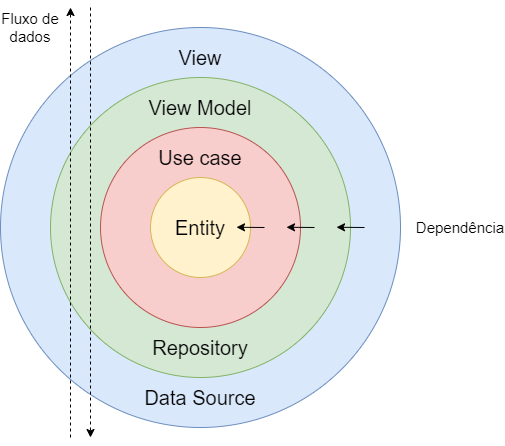
\includegraphics[scale=0.5]{clean-adapt.png}
  \caption{Diferença entre dependência e fluxo de dados.}
  \label{fig:cleanadapt}
\end{figure}

Note que as dependências estão sempre apontando para o interior. Levando em consideração a explicação de como as fronteiras das camadas são passadas através da inversão de dependências, o diagrama de pacotes da \Figura{fig:package} possui a modelagem mais abstrata e de maior alto nível da arquitetura do aplicativo. 

% imagem do diagrama de pacotes 
\begin{figure}[!htb]
  \centering
  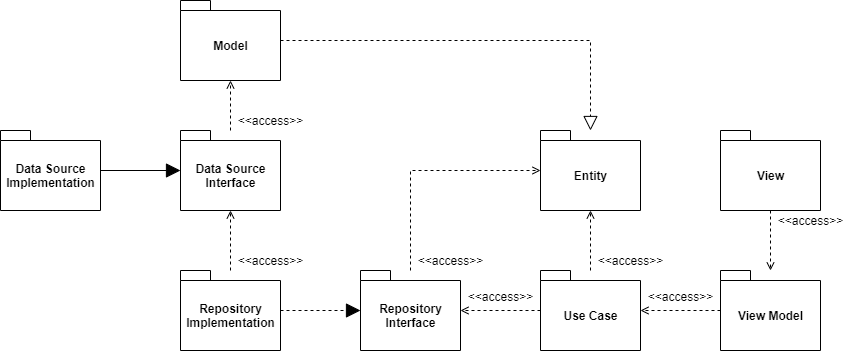
\includegraphics[scale=0.5]{Diagrama de pacotes.png}
  \caption{Diagrama de pacotes do aplicativo.}
  \label{fig:package}
\end{figure}

Para que a associação do diagrama da \Figura{fig:package} com as camadas e regras de dependência da \Figura{fig:cleanadapt} sejam melhor visualizadas, a \Figura{fig:package2} representa as camadas da arquitetura limpa com as mesmas colorações por cima do diagrama de pacotes.

\begin{figure}[!htb]
  \centering
  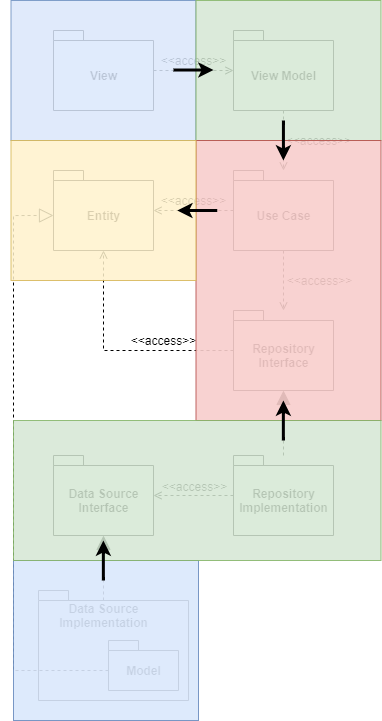
\includegraphics[scale=0.43]{package-adapt.png}
  \caption{Diagrama de pacotes com as colorações das camadas da arquitetura limpa.}
  \label{fig:package2}
\end{figure}

Com todos diagramas mostrados anteriormente modelados, o diagrama de classes foi feito com base nos outros e pode ser visualizado na \Figura{fig:diagramadeclasses}. Como alguns diagramas ficaram grandes, a visualização deles fica impossibilitada nas páginas deste trabalho, por isso, visualize a pasta figuras\footnote{Disponível em: <https://github.com/Feggah/tcc/tree/main/docs/figuras>. Acesso em: 21 out. 2021.} no repositório do \textit{GitHub} para uma visão mais detalhada.

\begin{figure}[!htb]
  \centering
  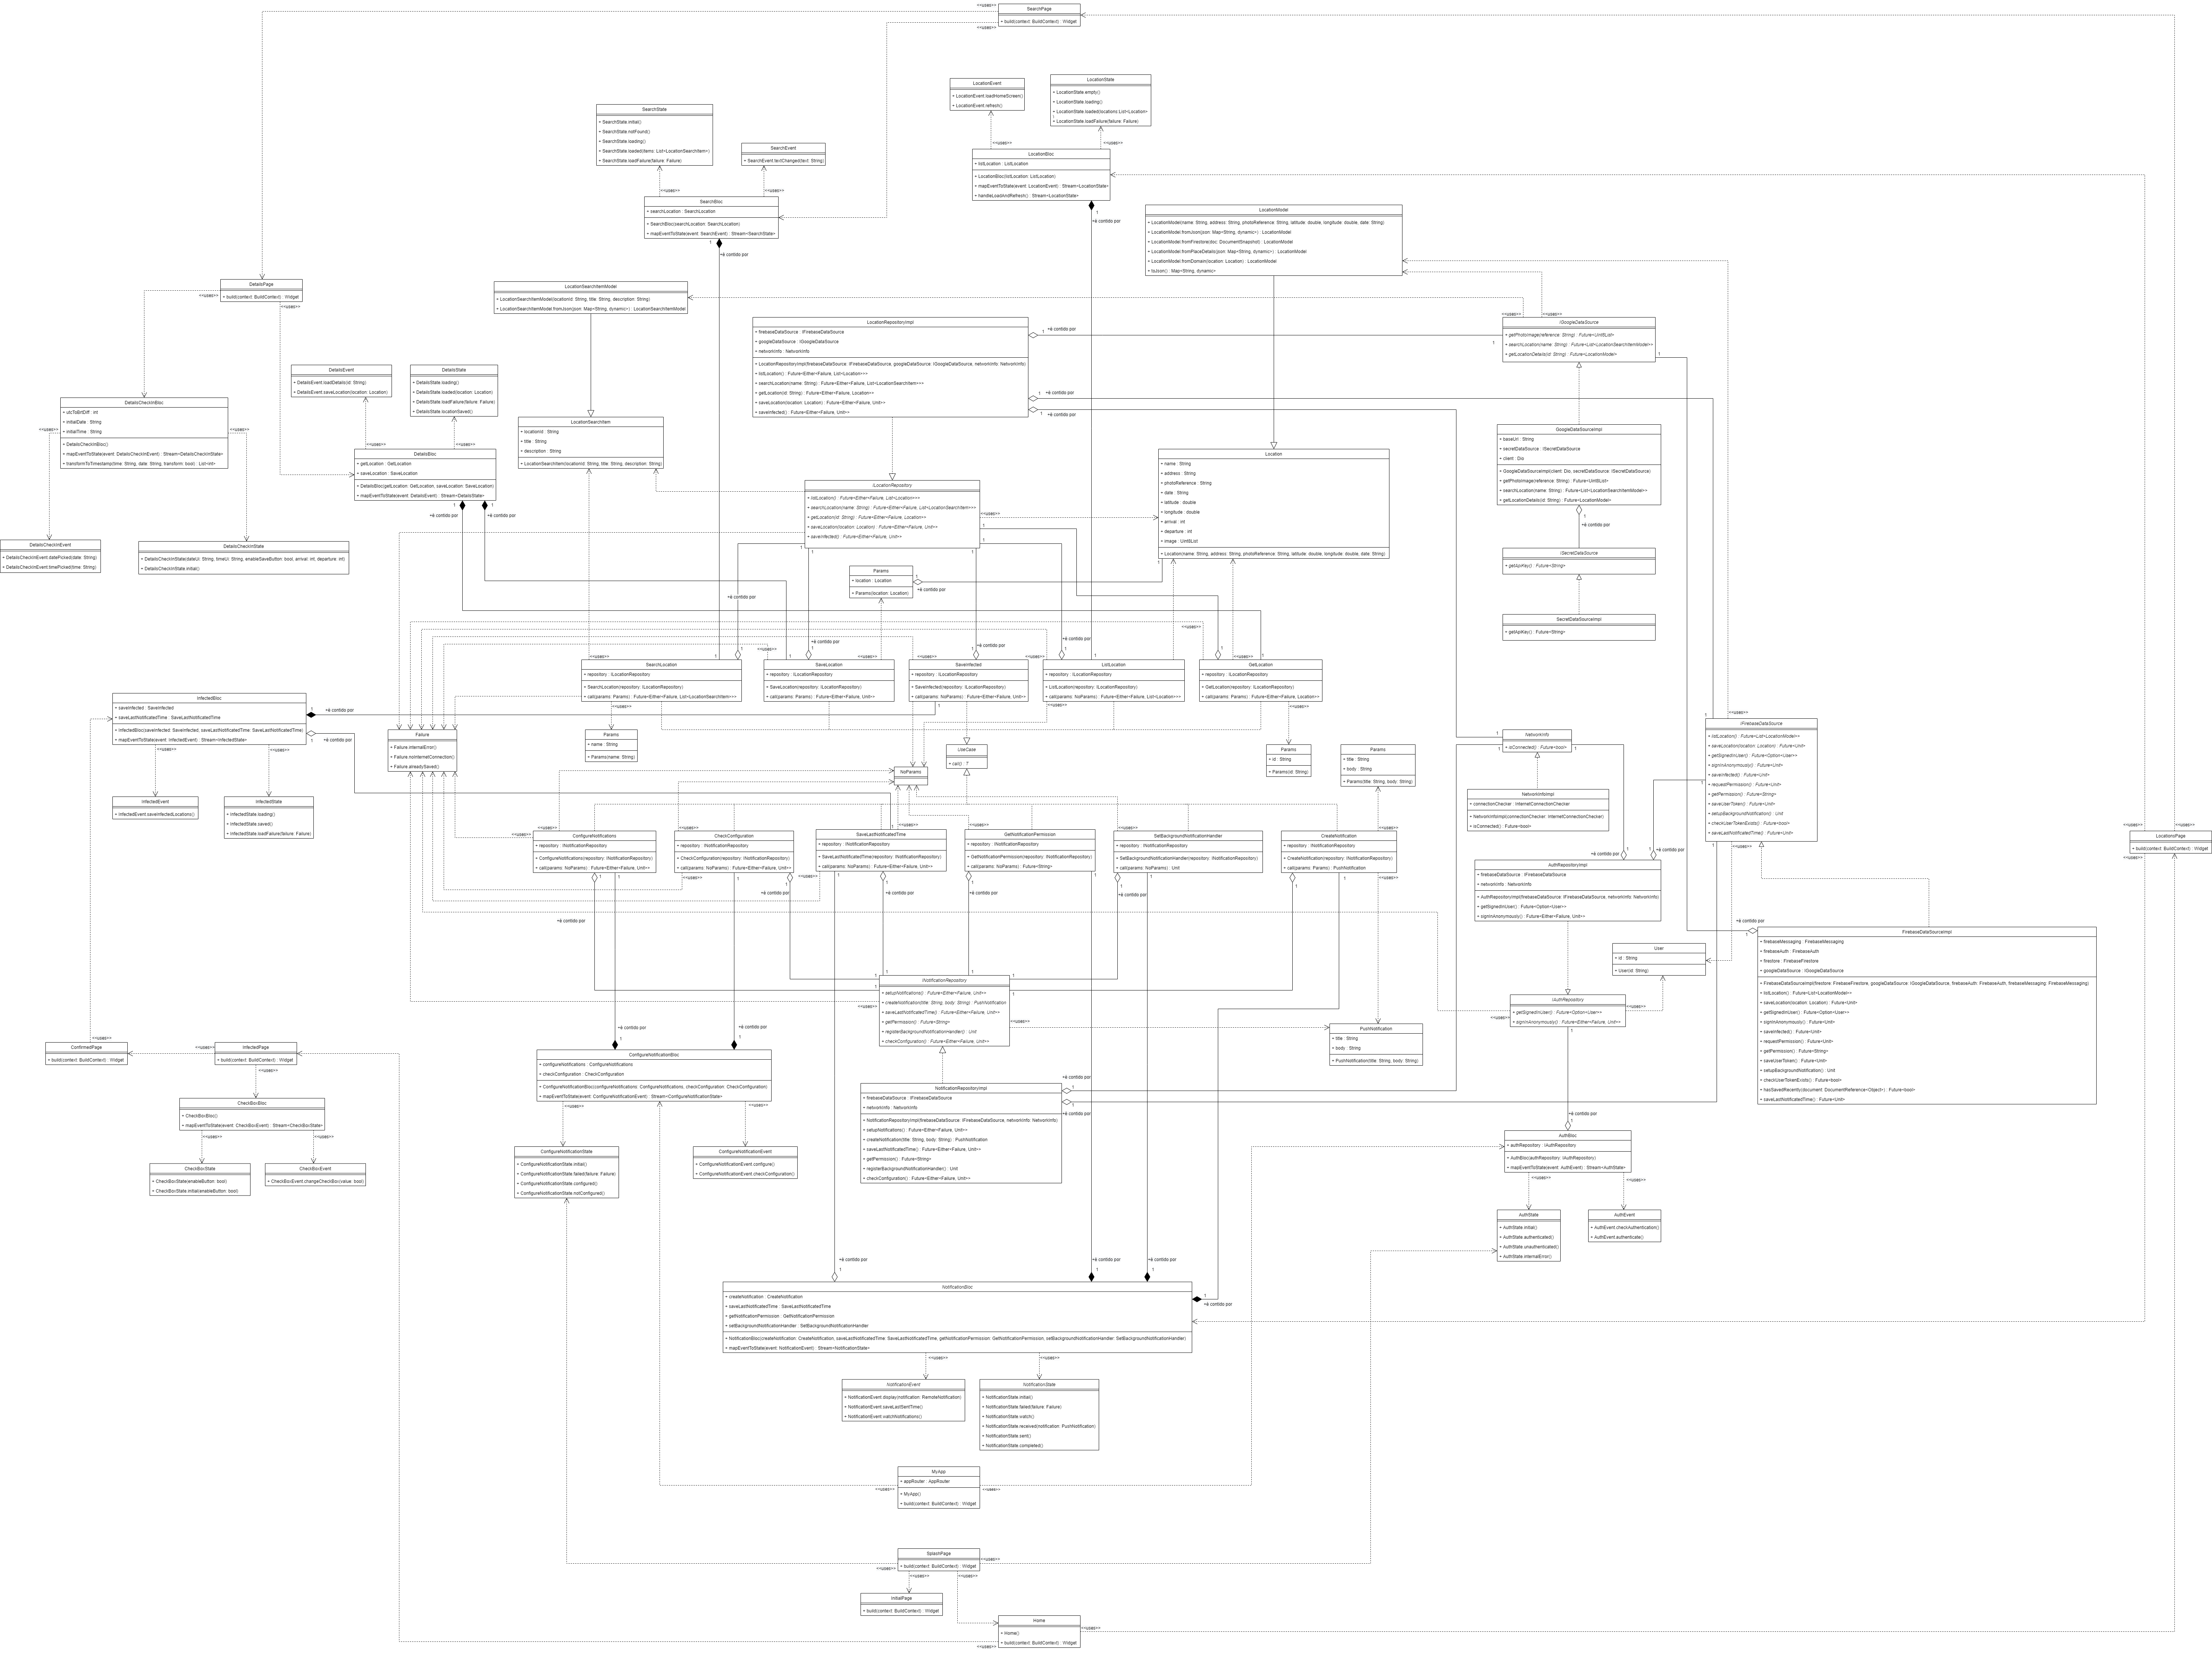
\includegraphics[scale=0.075]{Diagrama de classes.png}
  \caption{Diagrama de classes do aplicativo.}
  \label{fig:diagramadeclasses}
\end{figure}

\subsection{Modelagem de dados}\label{sec:modelagemdedados}
O sistema de rastreamento de dados necessita apenas de algumas informações persistidas sobre os usuários para que a análise de encontro entre eles seja efetuada com sucesso. 

Para cada usuário deverá ser armazenado os locais visitados e um identificador aleatório que possibilita o envio de notificações ao seu dispositivo móvel. Para isso, será utilizado uma coleção no \textit{Firestore} chamada \textit{users}. Nela serão armazenados múltiplos documentos, em que cada um representa um usuário. Em cada documento haverá o \textit{token} e a subcoleção dos locais visitados.

Além disso, dois campos opcionais também serão necessários. Um deles garantirá que o usuário não seja notificado múltiplas vezes em um curto período de tempo, o outro garantirá que ele não consiga se declarar como infectado múltiplas vezes dentro do período de 14 dias. O nome desses dois campos são respectivamente chamados de \textit{lastNotified} e \textit{lastSaved}.

Os documentos que representam os locais visitados serão compostos por alguns valores de retorno da API do \textit{Google}, que são os campos endereço, latitude, longitude, nome e o ID da foto. Para armazenar o horário que o usuário esteve no local, serão utilizados campos no formato \textit{timestamp} do horário de chegada e de saída que forem preenchidos pelo usuário na interface do aplicativo.

Os locais considerados como infectados serão armazenados em outra coleção com o objetivo de diminuição de profundidade da estrutura do BD, resultando em menos requisições de leitura. A consequência disso é que o tempo de processamento do algoritmo de análise de rastreamento e os custos da nuvem diminuirão, porque será necessário apenas uma requisição de leitura para obter todos os locais infectados e o valor cobrado é diretamente relacionado com o número de requisições efetuadas.

Essa coleção tem o nome \textit{infected} e cada um de seus documentos representam um local, contendo o horário, latitude e longitude do local classificado como infectado.

Como resultado desse racional apresentado acima, a modelagem da \Figura{fig:modelagemfirestore} representa a estrutura e todos atributos obrigatórios e opcionais de cada documento.

\begin{figure}[!htb]
  \centering
  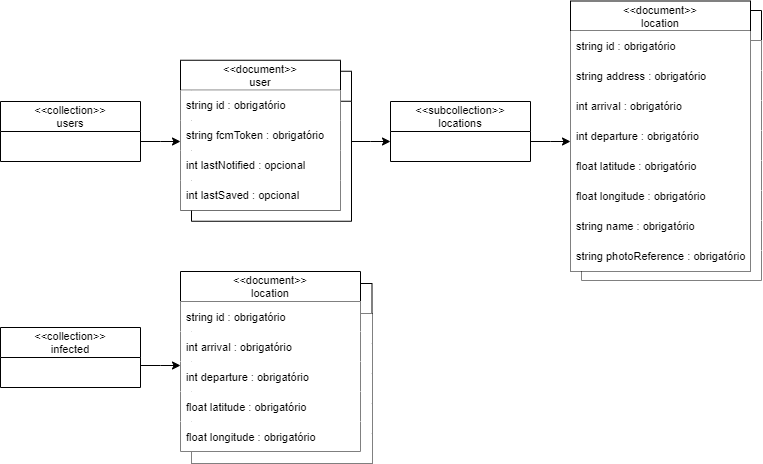
\includegraphics[scale=0.59]{Modelagem banco de dados.png}
  \caption{Modelagem do banco de dados não relacional.}
  \label{fig:modelagemfirestore}
\end{figure}

\section{Interfaces de usuário do aplicativo}\label{sec:uiux}
O \textit{design} das interfaces do aplicativo foi criado utilizando o \textit{Figma}, que é um editor online gratuito de gráficos vetoriais com ênfase na prototipagem de interfaces gráficas. Todos protótipos de tela construídos podem ser visualizados na página do projeto\footnote{Disponível em: <https://www.figma.com/file/x11PMoHwniQ0e1Jb6T6LRk/TCC>. Acesso em: 23 out. 2021.} dentro da ferramenta. 

As principais telas do aplicativo são as que estão diretamente associadas à uma das funcionalidades da Tabela \ref{tab:tabelaf} e representadas pelo diagrama de casos de uso da \Figura{fig:usecasesdiagram}, que são as telas de listagem, busca e visualização de locais e a de declaração de caso de infecção. Os protótipos das quatro telas podem ser visualizados na \Figura{fig:principaistelas}.

\begin{figure}[!htb]
  \centering
  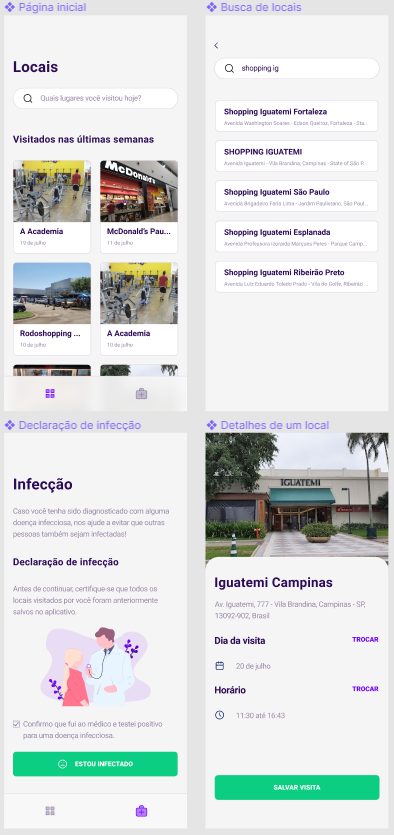
\includegraphics[scale=0.8]{interface-principais-telas.png}
  \caption{Protótipo das principais telas do aplicativo móvel.}
  \label{fig:principaistelas}
\end{figure}

Além das quatro telas principais, existem algumas variações das mesmas em casos de erro, falta de conexão com a \textit{Internet} e páginas de \textit{feedback} para alguma ação do usuário. Por exemplo, quando o usuário se auto declara como infectado, ele visualizará uma página de confirmação informando que o processamento foi concluído com sucesso.

\section{Implementação}\label{sec:implementacao}

As tarefas necessárias para conclusão do projeto foram criadas no formato de \textit{issues} no repositório do \textit{GitHub}. Cada issue foi classificada entre \textit{feature}, \textit{release}, \textit{diagram} e \textit{documentation} através de rótulos adicionados à elas.

O rótulo de \textit{release} significa que aquela \textit{issue} será concluída no momento que uma nova versão do sistema seja lançada. Isso também significa que uma \textit{release} contém várias \textit{issues} do tipo \textit{feature} que devem ser concluídas primeiramente.

Um exemplo de \textit{release} foi o lançamento do \Sigla{\textit{Minimum viable product}}{MVP}, que continha como pré-requisito a conclusão de todas as \textit{issues} que representavam as funcionalidades levantadas na Seção \ref{sec:requisitos}. A \Figura{fig:issuemvp} é um \textit{printscreen} que mostra como foi estruturada as \textit{issues} do repositório.

\begin{figure}[!htb]
  \centering
  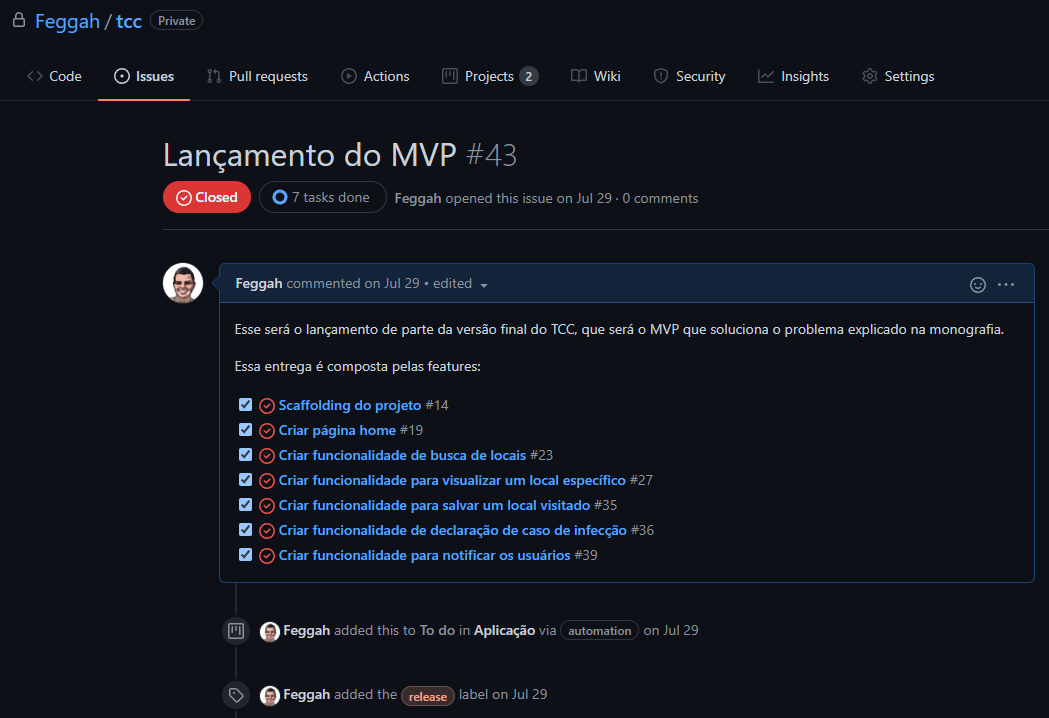
\includegraphics[scale=0.57]{mvp-issue.png}
  \caption{\textit{Printscreen} da \textit{issue} de lançamento do MVP.}
  \label{fig:issuemvp}
\end{figure}

Todas as \textit{issues} seguem esse mesmo modelo: possuem um título, descrição do que deve ser feito e um rótulo classificando qual o seu tipo.

O rótulo \textit{feature} representa uma funcionalidade a ser implementada no sistema. Essa funcionalidade não deve necessariamente representar uma relação um para um com as funcionalidades levantadas na Seção \ref{sec:requisitos}, ou seja, elas podem ser quebradas em entregas menores.

O rótulo \textit{documentation} está relacionado a tarefas de desenvolvimento do texto da monografia. Por exemplo, uma \textit{issue} que representa o desenvolvimento de um dos capítulos deste trabalho.

A última classificação, o rótulo \textit{diagram}, representa tarefas que estavam relacionadas a modelagem dos diagramas criados para este trabalho. No caso desse rótulo, foi utilizado uma \textit{issue} para cada tipo de diagrama, por exemplo, a \textit{issue} sobre o diagrama de atividades representava a modelagem dos seis diagramas criados. 

Para que a visualização e progresso das \textit{issues} fosse melhor visualizado, foi utilizado um quadro \textit{Kanban} oferecido nativamente pelo \textit{GitHub}, que são chamados de projetos. Foram criados dois projetos, um representando a implementação de todo o sistema e o outro o desenvolvimento da monografia e assuntos relacionados.

Os dois quadros \textit{Kanbans} foram divididos em três colunas: \textit{To do}, \textit{in progress} e \textit{done}. As \textit{issues} que estavam dentro de cada quadro eram movidas conforme o seu estado mudava em relação a coluna que ela estava inserida. Por exemplo, a \Figura{fig:kanbanmono} representa o estado do quadro da monografia durante o desenvolvimento desta seção.

\begin{figure}[!htb]
  \centering
  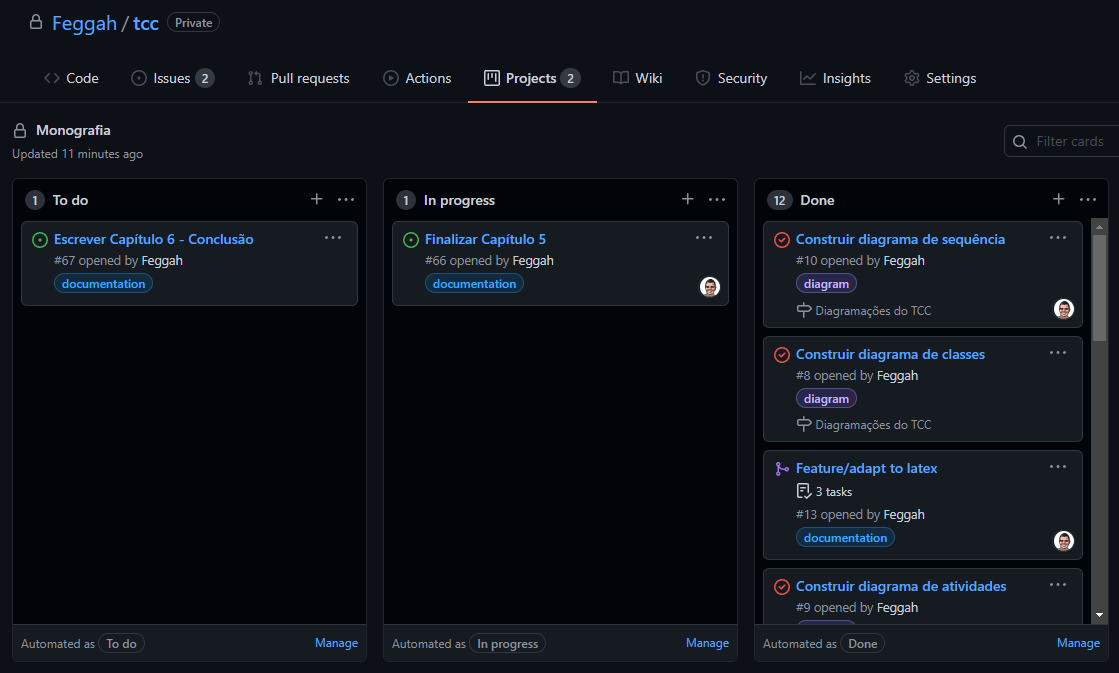
\includegraphics[scale=0.53]{kanban-github.png}
  \caption{\textit{Printscreen} do quadro \textit{Kanban} da monografia.}
  \label{fig:kanbanmono}
\end{figure}

Como explicado na Seção \ref{sec:Git}, o fluxo de trabalho escolhido para o processo de desenvolvimento do sistema foi o \textit{GitFlow}. Por conta disso, o repositório possui duas ramificações de longa vida, a \textit{main} e a \textit{develop}.

Para exemplificar o fluxo completo do \textit{GitFlow} na prática, a \Figura{fig:cfpr} possui um exemplo de \textit{pull request} para a ramificação \textit{develop}.

\begin{figure}[!htb]
  \centering
  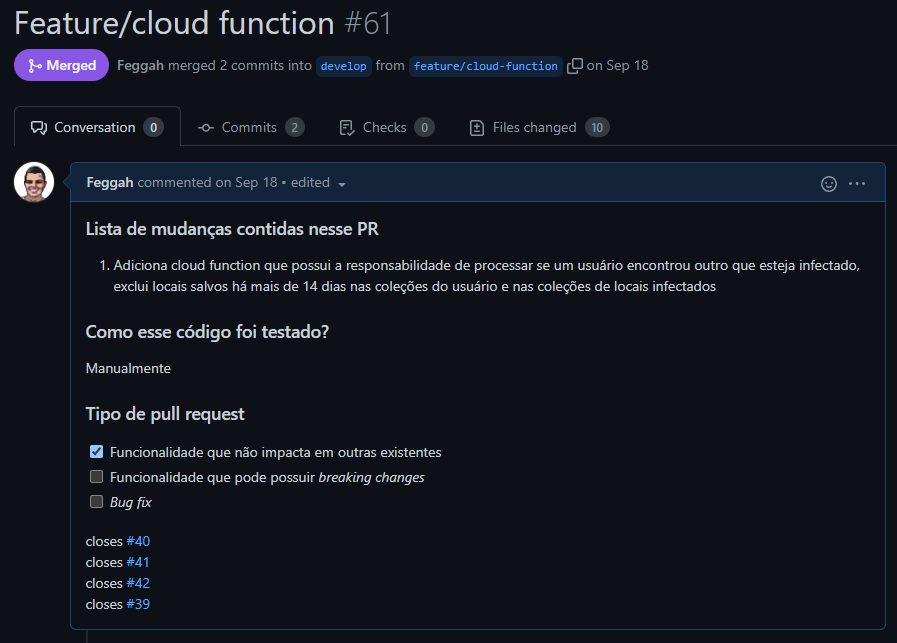
\includegraphics[scale=0.65]{pr-to-develop-example.png}
  \caption{\textit{Printscreen} de exemplo de um \textit{pull request} do repositório.}
  \label{fig:cfpr}
\end{figure}

Depois de algumas iterações de funcionalidades mescladas na ramificação \textit{develop}, a ramificação \textit{release} é criada a partir da \textit{develop} e são criados dois \textit{pull requests}, um para a \textit{main} e outro para a \textit{develop}. A \Figura{fig:releasemainpr} representa o \textit{pull request} para a main e a \Figura{fig:releasedeveloppr} para a \textit{develop}.

\begin{figure}[!htb]
  \centering
  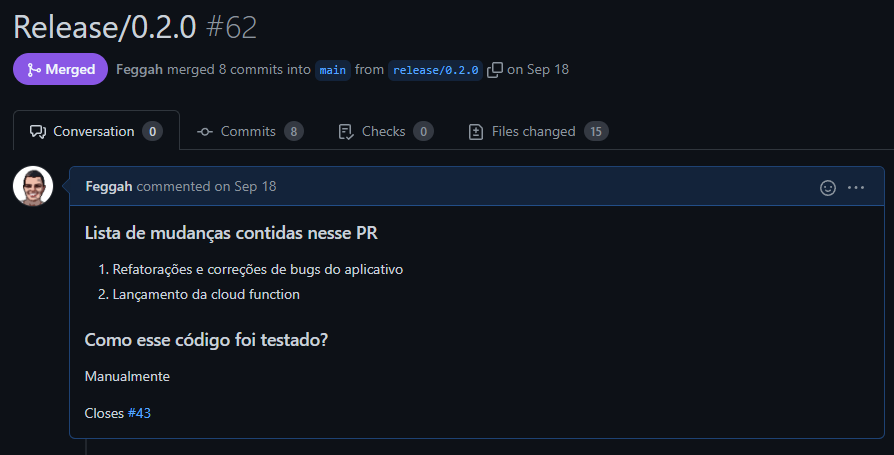
\includegraphics[scale=0.65]{pr-release-to-main.png}
  \caption{\textit{Printscreen} de exemplo de um \textit{pull request} da ramificação \textit{release} para \textit{main} do repositório.}
  \label{fig:releasemainpr}
\end{figure}

\begin{figure}[!htb]
  \centering
  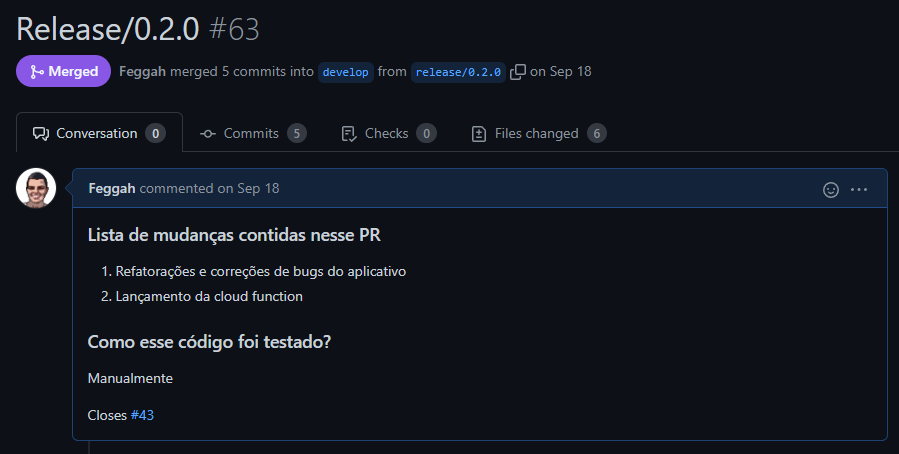
\includegraphics[scale=0.65]{pr-release-to-develop.png}
  \caption{\textit{Printscreen} de exemplo de um \textit{pull request} da ramificação \textit{release} para \textit{develop} do repositório.}
  \label{fig:releasedeveloppr}
\end{figure}

Com isso, a ramificação principal do repositório possui as novas funcionalidades desenvolvidas e uma nova versão está pronta para ser lançada. O lançamento de versão é feito adicionando uma \textit{tag}, que fixa um ponto histórico no repositório e representa uma versão da aplicação.

Com a nova \textit{tag} criada, um novo lançamento é feito através da funcionalidade de \textit{releases} do \textit{GitHub}. Uma \textit{release} contém título, descrição, a \textit{tag} que está associada à ela e arquivos que possam fazer parte desse lançamento. No caso do aplicativo, uma release contém o arquivo \Sigla{\textit{Android Package}}{APK} que pode ser baixado e instalado nos dispositivos. A \Figura{fig:currentreleases} representa os lançamentos feitos no repositório.

\begin{figure}[!htb]
  \centering
  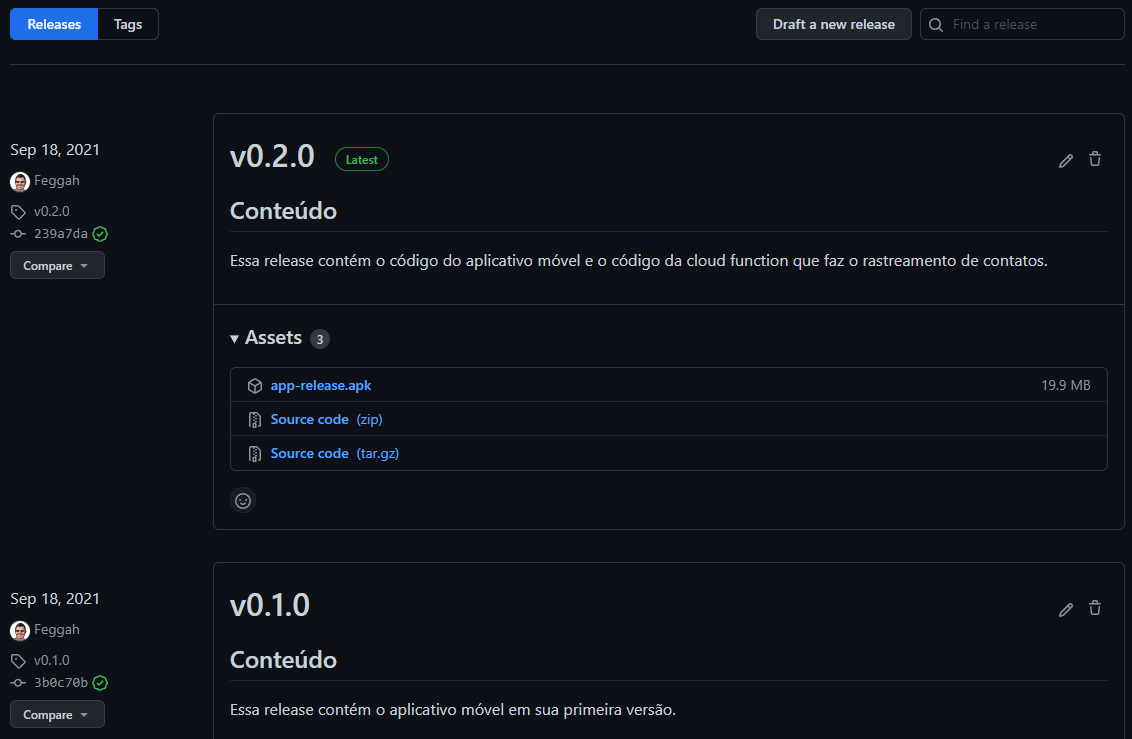
\includegraphics[scale=0.53]{repo-releases.png}
  \caption{\textit{Printscreen} das \textit{releases} do repositório.}
  \label{fig:currentreleases}
\end{figure}

Além do fluxo usual de incremento de funcionalidades, algumas correções pontuais podem ser feitas na versão que já está na ramificação principal através de ramificações denominadas de \textit{hotfix}. A \Figura{fig:hotfixpr} representa um exemplo desse tipo de modificação.

\begin{figure}[!htb]
  \centering
  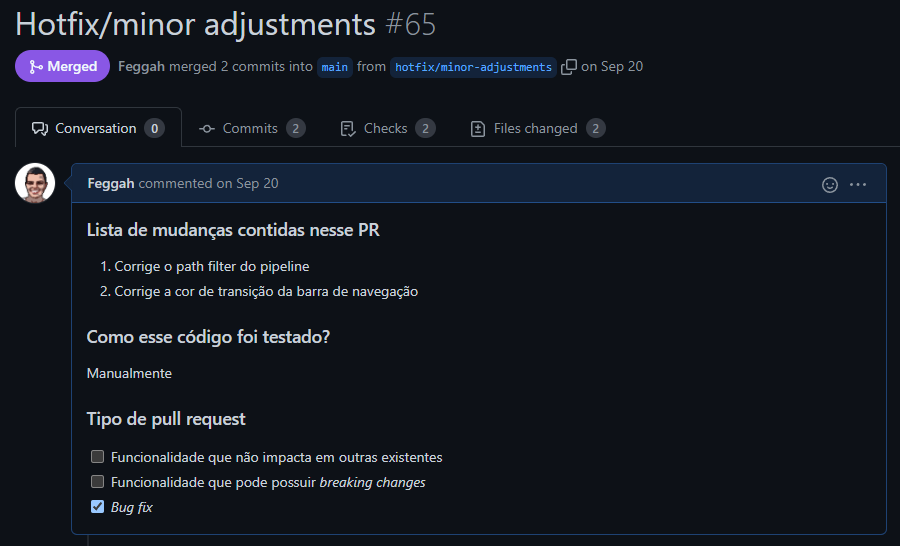
\includegraphics[scale=0.65]{pr-hotfix.png}
  \caption{\textit{Printscreen} de exemplo de um \textit{pull request} de \textit{hotfix}.}
  \label{fig:hotfixpr}
\end{figure}

Como o fluxo de trabalho escolhido utiliza o modelo de \textit{pull requests}, é importante que em cada um rode os testes automatizados, a fim de garantir que as novas modificações não estão quebrando o comportamento de funcionalidades antigas.

Para isso, foi desenvolvido um \textit{pipeline} utilizando as \textit{GitHub Actions}. Esse \textit{pipeline} roda todos os testes quando um novo \textit{pull request} é aberto e quando são feitos novos \textit{commits} na ramificação principal do repositório. A \Figura{fig:pipelineci} exemplifica os testes automatizados que foram ativados no evento de \textit{commit} da ramificação principal.

\begin{figure}[!htb]
  \centering
  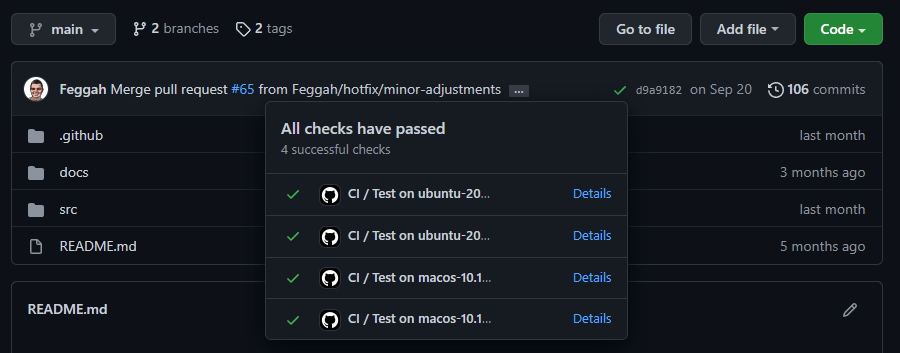
\includegraphics[scale=0.65]{pipeline.png}
  \caption{\textit{Printscreen} dos testes automatizados de \textit{commit} na ramificação principal.}
  \label{fig:pipelineci}
\end{figure}

Durante a implementação do aplicativo, a estrutura de pastas e arquivos reflete diretamente o diagrama de pacotes que foi apresentado na Seção \ref{sec:modelagem}. Existem quatro principais pastas: \textit{data}, \textit{domain}, \textit{presentation} e \textit{shared}.

\begin{figure}[!htb]
  \centering
  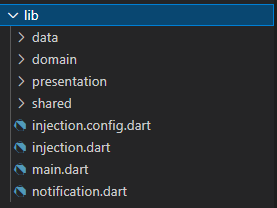
\includegraphics[scale=0.8]{lib-folder-structure.png}
  \caption{\textit{Printscreen} da estrutura de pastas do aplicativo.}
\end{figure}

A pasta \textit{data} contém as implementações dos repositórios, os modelos que são responsáveis pelas conversões entre a entidade interna do aplicativo e a sua representação externa em \textit{frameworks} ou bibliotecas terceiras, e os \textit{datasources}, que são responsáveis por se comunicarem com a \textit{Internet}.

A pasta \textit{domain} contém as entidades da aplicação, as interfaces de repositórios e os casos de uso. Essa pasta é a que deve sofrer menos alterações com o passar do tempo, porque não depende de \textit{frameworks} ou outros fatores que mudam com frequência.

A pasta \textit{presentation} contém as \textit{viewmodels}, a \textit{view} e as rotas do aplicativo. As rotas são utilizadas para fazer a navegação entre as diferentes telas. A \textit{view} contém a definição da interface com os usuários, ou seja, todos os protótipos criados no \textit{Figma} e citados na Seção \ref{sec:uiux}. As \textit{viewmodels} contém a lógica de apresentação das telas, sendo responsável por receber eventos e emitir estados que causam o recarregamento das interfaces para o estado desejado.

A pasta \textit{shared} contém arquivos que são compartilhados entre diversas camadas. Esses arquivos representam as exceções, as possíveis falhas, extensões de bibliotecas terceiras, a implementação de checagem de conectividade com a \textit{Internet} e a interface dos casos de uso.

A visão das pastas expandidas é representada pela \Figura{fig:folders}.

\begin{figure}[!htb]
  \centering
  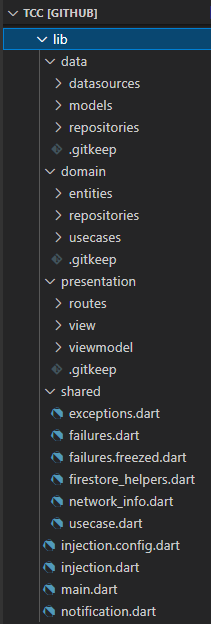
\includegraphics[scale=0.8]{app-folders.png}
  \caption{\textit{Printscreen} da estrutura de pastas expandidas do aplicativo.}
  \label{fig:folders}
\end{figure}

O aplicativo possui uma extensa lista de dependências em bibliotecas de terceiros que foram importadas para cumprir algum objetivo específico. As principais dependências do aplicativo são:

\begin{itemize}
  \item Bibliotecas do \textit{Firebase}, que são alguns \Sigla{\textit{Software Development Kit}}{SDK} que fazem a comunicação com as APIs do \textit{Firebase};
  \item \textit{Flutter\underline{\space}bloc}, que é um pacote para gerenciamento de estados;
  \item \textit{Dartz}, que é uma biblioteca que introduz programação funcional ao \textit{Dart};
  \item \textit{Dio}, que é uma biblioteca para fazer requisições HTTP;
  \item \textit{Get\underline{\space}it}, que é uma biblioteca para utilização do padrão de projeto \textit{Service Locator} para \textit{Dart} e \textit{Flutter}. Esse padrão de projeto é usado para encapsular os processos envolvidos na obtenção de um serviço com uma forte camada de abstração;
  \item \textit{Equatable}, que facilita a comparação de equalidade entre objetos;
  \item \textit{Freezed}, que é um gerador de código para classes imutáveis, introduzindo métodos auxiliares para seus objetos;
  \item \textit{Injectable}, que é um gerador de código para a biblioteca \textit{get\underline{\space}it};
\end{itemize}

Uma das partes mais importantes da implementação do aplicativo é a inversão de dependências, já explicado na subseção \ref{sec:D}. Essa inversão foi implementada utilizando a biblioteca \textit{injectable}.

Para fins de exemplificação, abaixo está exemplificado uma inversão de dependência entre a camada de domínio e a de dados, mais especificamente entre o caso de uso e o repositório.

A dependência do código está do repositório para o caso de uso e o fluxo de dados do caso de uso ao repositório. Para atigir isso, na camada de domínio foi definida a interface do repositório, que neste exemplo é a \textit{ILocationRepository}, representada pela \Figura{fig:locationrepository}.

\begin{figure}[!htb]
  \centering
  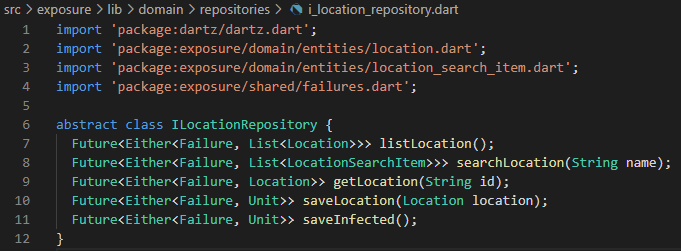
\includegraphics[scale=0.7]{ilocationrepository.png}
  \caption{\textit{Printscreen} da interface \textit{ILocationRepository}.}
  \label{fig:locationrepository}
\end{figure}

Na mesma camada temos o caso de uso \textit{ListLocation}, representado na \Figura{fig:listlocation}, que depende da interface \textit{ILocationRepository}. Essa dependência não fere os princípios da arquitetura limpa porque ambos estão na mesma camada.

\begin{figure}[!htb]
  \centering
  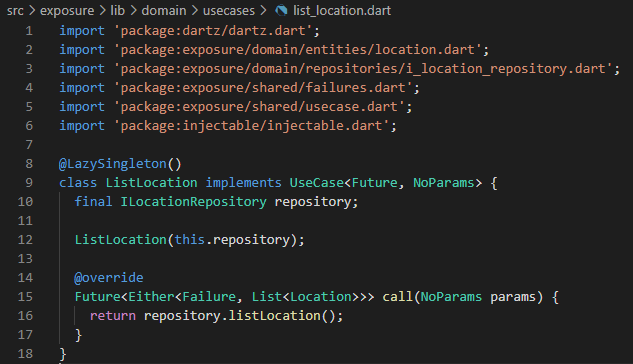
\includegraphics[scale=0.7]{listlocation.png}
  \caption{\textit{Printscreen} do caso de uso \textit{ListLocation}.}
  \label{fig:listlocation}
\end{figure}

Para que a inversão de dependência ocorra, em tempo de execução o atributo \textit{repository} da classe \textit{ListLocation} receberá uma instância da classe \textit{LocationRepositoryImpl} no lugar da \textit{ILocationRepository}. Isso será possível por conta do princípio de Liskov, explicado na subseção \ref{sec:liskov}.

A classe que implementa a interface \textit{ILocationRepository} é chamada de \textit{LocationRepositoryImpl} e está representada na \Figura{fig:locationimpl}. Note que o decorador da classe, que foi importado da biblioteca \textit{injectable}, faz com que as instâncias da classe sejam utilizadas nos atributos do tipo \textit{ILocationRepository}.

\begin{figure}[!htb]
  \centering
  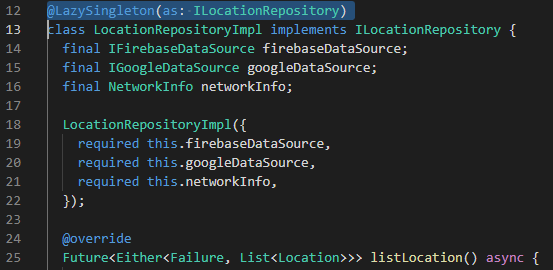
\includegraphics[scale=0.8]{locationimpl.png}
  \caption{\textit{Printscreen} da classe \textit{LocationRepositoryImpl}.}
  \label{fig:locationimpl}
\end{figure}

Esse mesmo modelo foi implementado em todas as fronteiras entre camadas, definindo a interface em uma camada e sua implementação em outra. Com isso, esse princípio da arquitetura limpa foi cumprido em todo aplicativo.

A implementação da \textit{cloud function} que faz a análise do rastreamento entre contatos é responsável por notificar os usuários que forem expostos à alguma doença. A notificação recebida por um dispositivo está exemplificada na \Figura{fig:appnotification}.

\begin{figure}[!htb]
  \centering
  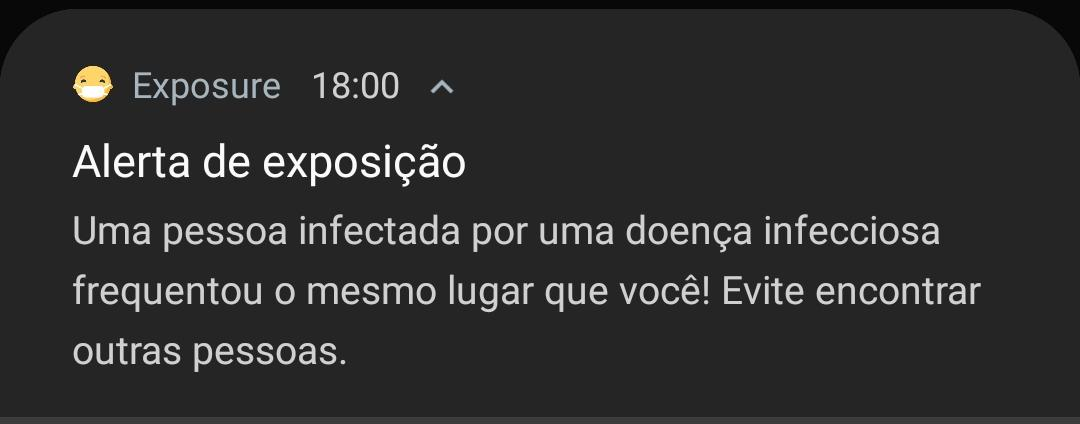
\includegraphics[scale=0.3]{app-notification.jpeg}
  \caption{\textit{Printscreen} da notificação recebida no dispositivo celular.}
  \label{fig:appnotification}
\end{figure}

Um usuário deverá ser notificado se:

\begin{itemize}
  \item A latitude e longitude dos locais salvos são as mesmas. Isso evita falsos positivos em locais com o mesmo nome mas em localizações diferentes. Por exemplo, franquias de uma empresa que estão localizadas em cidades diferentes;
  \item O horário de chegada do usuário é menor que o horário de saída do infectado;
  \item O horário de chegada do infectado é menor que o horário de saída do usuário sendo analisado;
\end{itemize}

Se todas as condições forem verdadeiras, utiliza-se o \textit{fcmToken}, explicado anteriormente na subseção \ref{sec:modelagemdedados}, do documento que representa o usuário para enviar uma notificação ao seu dispositivo. O trecho de código da \Figura{fig:cfscript} referente ao \textit{script} da \textit{cloud function} representa essa análise.

\begin{figure}[!htb]
  \centering
  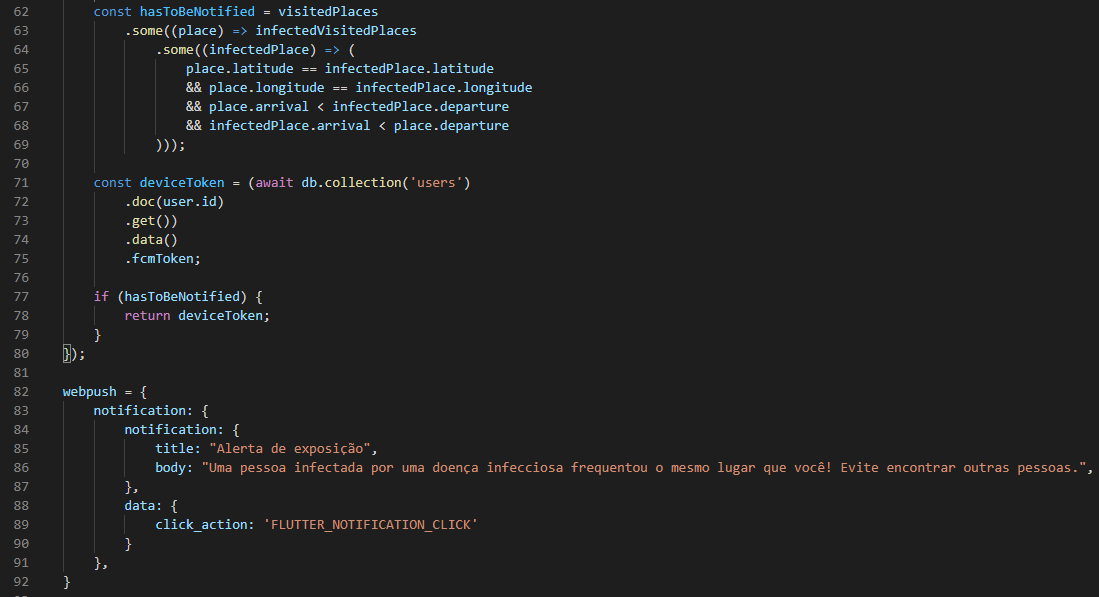
\includegraphics[scale=0.55]{cloudfunction-analysis.png}
  \caption{\textit{Printscreen} do trecho de código da \textit{cloud function}.}
  \label{fig:cfscript}
\end{figure}

As \textit{cloud functions} são definidas a partir de uma sintaxe em que é especificado o evento e o caminho da coleção que serão utilizados para ativá-la. Os possíveis eventos são \textit{OnCreate}, \textit{onUpdate}, \textit{onDelete} e \textit{onWrite}, que respectivamente correspodem aos eventos de criação, alteração, deleção ou todos anteriores.

As duas \textit{cloud functions} desenvolvidas neste trabalho são ativadas a partir de eventos de criação, uma na coleção de locais infectados e outra na subcoleção de locais salvos pelo usuário. A \Figura{fig:cfdeclaration} representa a declaração dessas funções.

\begin{figure}[!htb]
  \centering
  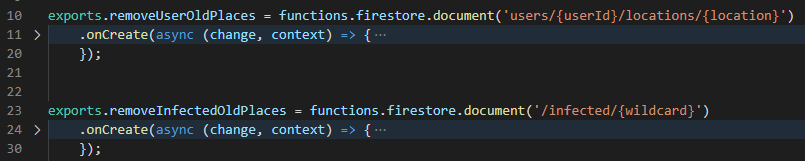
\includegraphics[scale=0.75]{cloudfunction-declaration.png}
  \caption{\textit{Printscreen} da declaração das \textit{cloud functions}.}
  \label{fig:cfdeclaration}
\end{figure}

Em relação a autenticação dos usuários, os IDs são criados aleatoriamente pelo serviço de autenticação do \textit{Firebase}. Como explicado em capítulos anteriores, a autenticação é feita de forma anônima e por conta disso a real identidade do usuário é preservada. Os únicos dados que podem ser extraídos dessa autenticação são a data de criação da conta, a data do último \textit{login} e o seu ID aleatório.

Todo mecanismo de autenticação é feito de forma transparente ao usuário no momento que ele inicia o aplicativo pela primeira vez. Caso o aplicativo seja deletado e instalado novamente, uma nova conta será criada, já que não há mecanismos de associação para definir a real identidade de cada usuário fora do sistema.
